\chapter{Задача о сдавливаниии цилиндрического идеально жесткопластического слоя}\label{ch:ch2}

\section{Постановка задачи и асимптотические разложения}\label{sec:ch2/sec1}

Пренебрегая начальными упругими деформациями, вязкостью и незначительным упрочнением, материал, имеющий плотность $\varrho$, полагается несжимаемым идеально жесткопластическим, удовлетворяющим тензорно линейным определяющим соотношениям и скалярному определяющему соотношению -- квадратичному критерию Мизеса-Генки $\sigma_{u} = \sigma_{s}$, где $\sigma_{u} = \sqrt{\utilde{s} : \utilde{s}}$ -- интенсивность напряжения, $\utilde{s}$ -- девиатор напряжения, $\sigma_{s}$ -- предел текучести.

Пусть течение происходит в области
\begin{equation}
  \Omega_{t} = \{0 \le r \le R(t) + h(t), -l(t) \le z \le l(t), 0 \le \theta < 2\pi\},
\end{equation}
с границей $\partial\Omega = \Gamma = \Gamma_{1} \cup \Gamma_{2} \cup \Gamma_{3}\cup \Gamma_{4}$, причем $h(t) \ll l(t)$ для любого $t \ge 0$. В начальный момент времени область, занятая материалом, имела вид
\begin{equation}
  \Omega_{0} = \{0 \le r \le R_{0} + h_{0}, -l_{0} \le z \le l_{0}, 0 \le \theta < 2\pi\}, \quad \partial\Omega_{0} = \Gamma_{0}
\end{equation}
поэтому в силу несжимаемости $(2R+h)hl=(2R_{0}+h_{0})h_{0}l_{0}$.

\begin{figure}[ht]
  \centerfloat{
    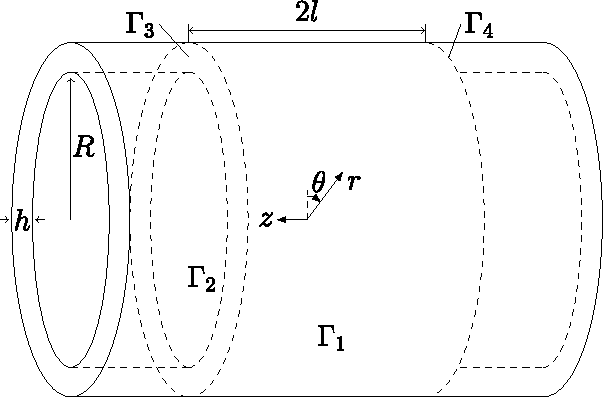
\includegraphics[width=0.6\linewidth]{./ch2/layer}
    }
    \caption{Представление цилиндрического слоя}
    \label{fig:ch2/layer}
\end{figure}
Скорость расширения внутреннего цилиндра обозначим $V$, поэтому кинематическое условие непротекания сквозь границы $\Gamma_{1}$ и $\Gamma_{2}$ имеет вид
\begin{equation}
  \label{eq:ch2/sec1/boundary/kinematic}
  v_{r}\lvert_{r=R} = V, \quad v_{r}\lvert_{r=R+h} = 0
\end{equation}
Касательная составляющая скорости (в данном случае $v_{z}$) на указанных границах идеальной среды, как известно, не задаётся.

В некоторый момент времени $0 < t < h_{0}/V = t_*$, где $t_*$ -- момент схлопывания слоя, относительно шести функций -- независимых компонент девиатора напряжений $s_{rr}$, $s_{rz}$ и $s_{\theta\theta}$, давления $p$ и компонент скорости $v_{r}$ и $v_{z}$ -- должна выполнятся замкнутая система уравнений динамической теории идеальной пластичности для цилиндрических координат:
\begin{subequations}
  \label{eqs:ch2/sec1/general}
  \begin{gather}
    \label{eqs:ch2/sec1/general/motion:1}
    -p_{,r}+s_{rr,r}+s_{rz,z}+\frac{s_{rr}-s_{\theta\theta}}{r} = \varrho \left(v_{r;t}+v_{r} v_{r,r} + v_{z} v_{r,z} \right)
    \\
    \label{eqs:ch2/sec1/general/motion:2}
    -p_{,z}+s_{rz,r}+\frac{s_{rz}}{r}-(s_{rr}+s_{\theta\theta})_{,z} = \varrho \left(v_{z;t}+v_{r} v_{z,r} + v_{z} v_{z,z} \right)
    \\
    \label{eqs:ch2/sec1/general/plasticity}
    s^2_{rr}+s^2_{\theta\theta}+s_{rr} s_{\theta\theta} + s^2_{rz}=\tau^2_{s}
    \\
    \label{eqs:ch2/sec1/general/coax:1}
    s_{rr} \frac{v_{r}}{r} = s_{\theta\theta} v_{r,r}
    \\
    \label{eqs:ch2/sec1/general/coax:2}
    s_{rr} (v_{r,z}+v_{z,r}) = 2 s_{rz} v_{r,r}
    \\
    \label{eqs:ch2/sec1/general/uncompress}
    v_{r,r}+\frac{v_{r}}{r}+v_{z,z} = 0
  \end{gather}
\end{subequations}
Кроме выполнения условия \cref{eq:ch2/sec1/boundary/kinematic} на жестких контактирующих поверхностях потребуем, что бы модуль касательного напряжения $s_{rz}$ достигал на границах $\Gamma_{1}$ и $\Gamma_{2}$ своего максимального значения:
\begin{equation}
  \label{eq:ch2/sec1/boundary/force}
  \lvert s_{rz}\lvert_{r=R} = \lvert s_{rz}\lvert_{r=R+h} = \mu \tau_{s}, \quad 0 < \mu \le 1,
\end{equation}
где $\mu$ -- шероховатость пресса. Абсолютной шероховатости, или полному сцеплению пресса с материалом, соответствует значение $\mu = 1$.

В реальном процессе сжатия слоя границы $\Gamma_{3}$ и $\Gamma_{4}$, естественно, свободны от напряжений, однако в математической постановке рассматриваемой здесь краевой задачи в её классическом варианте данное условие не ставится. Поэтому других, помимо \cref{eq:ch2/sec1/boundary/kinematic, eq:ch2/sec1/boundary/force}, граничных условий в задаче не предполагается, а область вблизи границ $\Gamma_{3}$ и $\Gamma_{4}$(на расстояниях порядка $h$) трактуется как зона краевого эффекта.

Введем малый параметр $\alpha = \frac{h(t)}{l(t)} \ll 1$ и проведем разложение всех неизвестных величин, входящих в систему уравнений \cref{eqs:ch2/sec1/general}, в ряды по целым степеням параметра:
\begin{subequations}
  \label{eqs:ch2/series}
  \begin{gather}
    v_{r}\left(r, z, t\right) = V \sum_{k=0}^{\infty}{\alpha^{k} \; \uindex{v}{k}_{r}}
    \\
    v_{z}\left(r, z, t\right) = V \sum_{k=-N}^{\infty}{\alpha^{k} \; \uindex{v}{k}_{z}}, \quad N \ge 1
    \\
    s_{ij}\left(r, z, t\right) = \tau_{s} \sum_{k=0}^{\infty}{\alpha^{k} \; \uindex{s}{k}_{ij}}, \quad (ij)\in\{rr, rz, \theta\theta\}
    \\
    p\left(r, z, t \right) = \tau_{s} \sum_{k=-M}^{\infty}{\alpha^{k} \; \uindex{p}{k}}, \quad M \ge 1
  \end{gather}
\end{subequations}
Коэффициенты рядов \cref{eqs:ch2/series} -- безразмерны и являются функциями безразмерных координат $\rho, \xi, \tau$ :
\begin{equation}
  \label{eq:ch2/coordinates}
  \rho = \frac{r-R}{h}, \quad \xi = \frac{z}{l}=\frac{\alpha z}{h}, \quad \tau = V \frac{t}{h}
\end{equation}
Наличие в \cref{eqs:ch2/series} членов $\alpha^{-n} \; \uindex{v}{-n}_{z}$ и $\alpha^{-m} \; \uindex{p}{-m}$ обусловлено стремлением $v_{r}$ и $p$ к бесконечности, при $\alpha\rightarrow 0$, что ясно из физических соображений. Также заметим, что область $\Omega$ содержит три геометрических размера: $h$, $l$ И $R$, и если отношеные первых двух образую малый параметр, то отнощшение двух последних может иметь любой ``промежуточный'' порядок малости:
\begin{equation}
  \label{eq:ch2/sec1/c}
  R/l = a \alpha^c, \quad c\in[0,1], \quad a=O(1)
\end{equation}
Обратимся к геометрическому условию несжимаемости и выразим малый параметр и координаты \cref{eq:ch2/coordinates} как эволюционные функции:
\begin{subequations}
  \begin{gather}
    \left(\left(2r+h\right)h l\right)^. = 0, \quad \dot{l} = \frac{2 V R l}{\left(2R + h\right)h}=\frac{2 V R/l}{\left(2R/l + \alpha\right)\alpha}=\frac{2 V a \alpha^c}{\left(2a \alpha^c + \alpha\right)\alpha}\nonumber
    \\
    \dot{\alpha} = \left(\frac{h}{l}\right)^. = \frac{\dot{h}l - h\dot{l}}{l^2} = -\frac{V\alpha}{h}\left(2-\frac{\alpha}{2a\alpha^c+\alpha}\right)
    \\
    \dot{\rho} = \left(\frac{r-R}{h}\right)^. = \frac{-\dot{R} h - \dot{h}\left(r-R\right)}{h^2} = \frac{V}{h}\left(\rho-1\right)
    \\
    \dot{\xi} = \left(\frac{z}{l}\right)^. = -\frac{z \dot{l}}{l^2} = -\frac{V\xi\alpha}{h}\left(1-\frac{\alpha}{2a\alpha^c+\alpha}\right)
    \\
    \dot{\tau} = \left(V \frac{t}{h}\right)^. = V \frac{h - t\dot{h}}{h^2} = \frac{V}{h} \left(1+\tau\right)
  \end{gather}
\end{subequations}
Подставляя выражения \cref{eqs:ch2/series} в систему \cref{eqs:ch2/sec1/general} и учитывая, что полная производная по времени представляется в виде
\begin{equation*}
  \uindex{v}{k}_{i;t} = \uindex{v}{k}_{i,\rho} \dot{\rho} + \uindex{v}{k}_{i,\xi} \dot{\xi} + \uindex{v}{k}_{i,\tau} \dot{\tau}
\end{equation*}
получим следующую систему:
\begingroup
\allowdisplaybreaks
\begin{subequations}
  \label{eqs:ch2/sec1/substituted}
  \begin{gather}
    \label{eqs:ch2/sec1/substituted/motion:1}
    \begin{multlined}
      -\sum_{k=-M}^{\infty}{\alpha^{k} \; \uindex{p}{k}_{,\rho}} + \sum_{k=0}^{\infty}{\alpha^{k}\left(
      \ \uindex{s}{k}_{rr,\rho} + \alpha \ \uindex{s}{k}_{rz,\xi} + \frac{\alpha}{\alpha\rho+a \alpha^c}\left(\ \uindex{s}{k}_{rr} - \uindex{s}{k}_{\theta\theta}\right)
      \right)} \unl{=} \frac{\varrho V^2}{\tau_{s}}\left(
      \sum_{k=0}^{\infty}\alpha^{k}\left(
      \uindex{v}{k}_{r,\rho} \left(\rho+1\right) -
      \uindex{v}{k}_{r,\xi} \xi\alpha\left(1-\frac{\alpha}{2a\alpha^c+\alpha}\right) \right. \unl[1]{+} \uindex{v}{k}_{r,\tau} \left(1+\tau\right) -
      \left(2-\frac{\alpha}{2a\alpha^c+\alpha}\right) \ \uindex{v}{k}_{r}
      \right) \unl{+}
      \left.
      \sum_{k=0}^{\infty}{\alpha^{k} \; \uindex{v}{k}_{r}} \sum_{k=0}^{\infty}{\alpha^{k} \; \uindex{v}{k}_{r,\rho}} +
      \sum_{k=-N}^{\infty}{\alpha^{k} \; \uindex{v}{k}_{z}} \sum_{k=0}^{\infty}{\alpha^{k+1} \; \uindex{v}{k}_{r,\xi}}
      \right)
    \end{multlined}
    \\
    \label{eqs:ch2/sec1/substituted/motion:2}
    \begin{multlined}
      -\sum_{k=-M}^{\infty}{\!\!\alpha^{k+1} \ \uindex{p}{k}_{,\xi}} \!+\!
      \sum_{k=0}^{\infty}{\alpha^{k}\!\left(
      \uindex{s}{k}_{rz,\rho} +
      \frac{\alpha}{\alpha\rho+a \alpha^c} \ \uindex{s}{k}_{rz} -
      \alpha\left(\ \uindex{s}{k}_{rr,\xi} + \uindex{s}{k}_{\theta\theta,\xi}\right)
      \right)} \unl{=}
      \frac{\varrho V^2}{\tau_{s}}\left(
      \sum_{k=-N}^{\infty}\alpha^{k}\left(
      \uindex{v}{k}_{z,\rho} \left(\rho+1\right) -
      \uindex{v}{k}_{z,\xi} \xi\alpha\left(1-\frac{\alpha}{2a\alpha^c+\alpha}\right) \right. \unl[1]{+} \uindex{v}{k}_{z,\tau} \left(1+\tau\right) -
      \left(2-\frac{\alpha}{2a\alpha^c+\alpha}\right) \ \uindex{v}{k}_{z}
      \right) \unl{+}
      \left.
      \sum_{k=0}^{\infty}{\alpha^{k} \; \uindex{v}{k}_{r}} \sum_{k=-N}^{\infty}{\alpha^{k} \; \uindex{v}{k}_{z,\rho}} +
      \sum_{k=-N}^{\infty}{\alpha^{k} \; \uindex{v}{k}_{z}} \sum_{k=-N}^{\infty}{\alpha^{k+1} \; \uindex{v}{k}_{z,\xi}}
      \right)
    \end{multlined}
    \\
    \label{eqs:ch2/sec1/substituted/plasticity}
    \begin{multlined}
      \left(\sum_{k=0}^{\infty}{\alpha^{k} \; \uindex{s}{k}_{rr}}\right)^2+
      \left(\sum_{k=0}^{\infty}{\alpha^{k} \; \uindex{s}{k}_{\theta\theta}}\right)\unl{+}
      \sum_{k=0}^{\infty}{\alpha^{k} \; \uindex{s}{k}_{rr}} \sum_{k=0}^{\infty}{\alpha^{k} \; \uindex{s}{k}_{\theta\theta}}+
      \left(\sum_{k=0}^{\infty}{\alpha^{k} \; \uindex{s}{k}_{rz}}\right)^2 = 1
    \end{multlined}
    \\
    \label{eqs:ch2/sec1/substituted/coax:1}
    \sum_{k=0}^{\infty}{\alpha^{k} \; \uindex{s}{k}_{rr}} \; \frac{\alpha}{\alpha\rho+a \alpha^c} \sum_{k=0}^{\infty}{\alpha^{k} \; \uindex{v}{k}_{r}} = \sum_{k=0}^{\infty}{\alpha^{k} \; \uindex{s}{k}_{\theta\theta}} \sum_{k=0}^{\infty}{\alpha^{k} \; \uindex{v}{k}_{r,\rho}}
    \\
    \label{eqs:ch2/sec1/substituted/coax:2}
    \sum_{k=0}^{\infty}{\alpha^{k} \; \uindex{s}{k}_{rr}} \left(
    \sum_{k=0}^{\infty}{\alpha^{k+1} \; \uindex{v}{k}_{r,\xi}} +
    \sum_{k=-N}^{\infty}{\alpha^{k} \; \uindex{v}{k}_{z,\rho}}
    \right) = 2 \sum_{k=0}^{\infty}{\alpha^{k} \; \uindex{s}{k}_{rz}} \sum_{k=0}^{\infty}{\alpha^{k} \; \uindex{v}{k}_{r,\rho}}
    \\
    \label{eqs:ch2/sec1/substituted/uncompress}
    \sum_{k=0}^{\infty}{\alpha^{k} \; \uindex{v}{k}_{r,\rho}} + \frac{\alpha}{\alpha\rho+a \alpha^c}\sum_{k=0}^{\infty}{\alpha^{k} \; \uindex{v}{k}_{r}} + \sum_{k=-N}^{\infty}{\alpha^{k+1} \; \uindex{v}{k}_{z,\xi}} = 0
  \end{gather}
\end{subequations}
\endgroup
Возникший в правой части уравнений \cref{eqs:ch2/sec1/substituted/motion:1, eqs:ch2/sec1/substituted/motion:2} коэффициент равен обратному числу Эйлера
\begin{equation*}
  \text{Eu}^{-1} = \frac{\varrho V^2}{\tau_{s}}.
\end{equation*}
Данная величина мала \todo{почему?}и как видно из её определения фиксирована. По сравнению с ней порядок малости $\alpha(t)$ при течении времени от 0 до $t_*$ растёт до бесконечности. Это позволяет записать
\begin{equation*}
  \text{Eu}^{-1} = O\left(\alpha^\beta(t)\right), \text{ причем } \beta \rightarrow 0 \text{ при } t \rightarrow t_*
\end{equation*}
Применительно к динамическому анализу интерес представляет $0 < \beta \le 2$. Отыскание решений проведем для целочисленных значений входящих в этот диапазон.

Обратимся к системе двух последних уравнений \cref{eqs:ch2/sec1/substituted/coax:2, eqs:ch2/sec1/substituted/uncompress}. Из них сразу следует, что $\uindex{v}{-N}_{r,\xi} = 0$ и $\uindex{v}{-N}_{r,\rho} = 0$, то есть $\uindex{v}{-N}_{z} = \uindex{g}{-N}_{v_{z}}(\tau)$ зависит только от $\tau$, обуславливая перемещение вдоль оси $z$ как абсолютно жесткого целого. Исключив данное движение из рассмотрения, можно принять $\uindex{v}{-N}_{z} = 0$. Аналогичные рассуждения применимы последовательно для $\uindex{v}{-N+1}_{z}$, затем $\uindex{v}{-N+2}_{z}$ и далее вплоть до $\uindex{v}{-2}_{z}$.
Учитывая, что первый ненулевой член продольной компоненты скорости $\uindex{v}{-1}_{z}$, и принимая, что $\beta \ge 1$ определим из уравнений \cref{eqs:ch2/sec1/substituted/motion:1, eqs:ch2/sec1/substituted/motion:2} порядок малости для функции давления $p$. Для $M \ge 2$ имеем:
\begin{equation*}
  -\uindex{p}{-M}_{,\rho} = 0, \quad -\uindex{p}{-M}_{,\xi} = 0 \text{ и, следовательно, } \ \uindex{p}{-M} = \uindex{p}{-M}_{0}(\tau)
\end{equation*}
Здесь $\uindex{p}{-M}_{0}$ -- гидростатическая постоянная, не дающая вклад в уравнение движения и однозначно определяемая заданием внешнего давления. Поэтому, без ограничения общности, можно считать, что $M=1$.

В указанном в \cref{eq:ch2/sec1/c} диапазоне параметра $c$ выделим три значения, соответствующие различным математическим и механическим смыслам:
\begin{itemize}
  \item $c=1$, когда радиусы цилиндров имеют порядок толщины слоя,
  \item $c=0$, когда радиусы цилиндров имеют порядок длины образующей,
  \item $0<c<1$, когда радиусы цилиндров имеют ``промежуточный'' порядок малости.
\end{itemize}
\section{Построение решения при радиусах цилиндров порядка толщины слоя}\label{sec:ch2/sec2}

При данном соотношении дробь $\frac{\alpha}{\alpha\rho+a \alpha^c}$ преобразуется к виду $\frac{1}{\rho+a}$ и не будет зависеть от $\alpha$, следовательно, будет являться величиной порядка $O(1)$.

\subsection{Переход от квазистатического к динамическому режиму деформирования}\label{subsec:ch2/sec2/sub1}

Рассмотрим случай $\beta=2$, который соответствует моменту перехода от квазистатического к динамическому режиму деформирования.

Положим $\text{Eu}^{-1} = C_2 \alpha^2$ и последовательно приравняем коэффициенты правых и левых частей уравнений системы \cref{eqs:ch2/sec1/substituted} при $a^{-1}$ и $\alpha^0$:
\begingroup
\allowdisplaybreaks
\begin{subequations}
  \label{eqs:ch2/sec2/sub1/main}
  \begin{gather}
    \label{eqs:ch2/sec2/sub1/-1/motion:2}
    -\uindex{p}{-1}_{,\rho} = 0
    \\
    \label{eqs:ch2/sec2/sub1/-1/coax:2}
    \uindex{s}{0}_{rr} \; \uindex{v}{-1}_{z,\rho} = 0
    \\
    \label{eqs:ch2/sec2/sub1/0/motion:1}
    -\uindex{p}{0}_{,\rho}+\uindex{s}{0}_{rr,\rho} + \left(\uindex{s}{0}_{rr}-\uindex{s}{0}_{\theta\theta}\right) / \left(\rho + a\right) = 0
    \\
    \label{eqs:ch2/sec2/sub1/0/motion:2}
    -\uindex{p}{-1}_{,\xi} + \uindex{s}{0}_{rz,\rho} + \uindex{s}{0}_{rz} / \left(\rho+a\right) = 0
    \\
    \label{eqs:ch2/sec2/sub1/0/plasticity}
    \left(\uindex{s}{0}_{rr}\right)^2 + \left(\uindex{s}{0}_{\theta\theta}\right)^2 + \uindex{s}{0}_{rr}\; \uindex{s}{0}_{\theta\theta} + \left(\uindex{s}{0}_{rz}\right)^2 = 1
    \\
    \label{eqs:ch2/sec2/sub1/0/coax:1}
    \uindex{s}{0}_{rr} \; \uindex{v}{0}_{r} / \left(\rho+a\right) = \uindex{s}{0}_{\theta\theta} \uindex{v}{0}_{r,\rho}
    \\
    \label{eqs:ch2/sec2/sub1/0/coax:2}
    \uindex{s}{0}_{rr} \; \uindex{v}{0}_{z,\rho} = 2 \uindex{s}{0}_{rz} \; \uindex{v}{0}_{r,\rho}
    \\
    \label{eqs:ch2/sec2/sub1/0/uncompress}
    \uindex{v}{0}_{r,\rho} + \uindex{v}{0}_{r} / \left(\rho+a\right) + \uindex{v}{-1}_{z,\xi} = 0
  \end{gather}
\end{subequations}
\endgroup
Граничные условия \cref{eq:ch2/sec1/boundary/kinematic, eq:ch2/sec1/boundary/force} при этом примут вид
\begin{equation}
  \label{eq:ch2/sec2/sub1/boundary/0}
  \uindex{v}{0}_{r}\lvert_{\rho=0} = 1,\quad \uindex{v}{0}_{r}\lvert_{\rho=1} = 0, \quad \lvert \uindex{s}{0}_{rz}\lvert_{\rho=0} = \lvert \uindex{s}{0}_{rz}\lvert_{\rho=1} = \mu
\end{equation}
Из уравнений \cref{eqs:ch2/sec2/sub1/-1/motion:2, eqs:ch2/sec2/sub1/-1/coax:2} вытекает
\begin{equation*}
  \uindex{p}{-1} = \uindex{f}{-1}_{p}(\xi, \tau), \quad \uindex{v}{-1}_{z} = \uindex{f}{-1}_{v_{z}}(\xi, \tau).
\end{equation*}
Подставив выражение $\uindex{v}{-1}_{z}$ в уравнение \cref{eqs:ch2/sec2/sub1/0/uncompress} и решив дифференциальное уравнение, получим выражение для $\uindex{v}{0}_{r}$:
\begin{equation*}
  \uindex{v}{0}_{r} = \left(\uindex{f}{0}_{v_{r}}(\xi, \tau) -\rho \left(a+\rho/2\right) \uindex{f}{-1}_{v_{z},\xi}\right) / \left(\rho+a\right)
\end{equation*}
Подстановка данного равенства в кинематические граничные условия \cref{eq:ch2/sec2/sub1/boundary/0} позволяет определить неизвестные функции интегрирования:
\begin{gather*}
  \uindex{f}{0}_{v_{r}} = a\\
  \uindex{f}{-1}_{v_{z}} = \frac{2a\xi}{2a+1} + \uindex{g}{-1}_{v_{z}}(\tau)
\end{gather*}
В силу симметрии задачи естественно требовать нечетности продольной компоненты скорости, что позволяет принять $\uindex{g}{-1}_{v_{z}}(\tau) = 0$. Окончательно получаем
\begin{gather}
  \label{sol:ch2/sec2/sub1/vz/-1}
  \uindex{v}{-1}_{z} = \uindex{f}{-1}_{v_{z}} = \frac{2a\xi}{2a+1}
  \\
  \label{sol:ch2/sec2/sub1/vr/0}
  \uindex{v}{0}_{r} =  \frac{a(1-\rho)(2a+\rho+1)}{(2a+1)(\rho+a)}
\end{gather}
Решая \cref{eqs:ch2/sec2/sub1/0/motion:2} относительно $\uindex{s}{0}_{rz}$ и используя силовые граничные условия \cref{eq:ch2/sec2/sub1/boundary/0} придем к
\begin{gather*}
  \uindex{s}{0}_{rz} = \left(\uindex{f}{0}_{s_{rz}}(\xi, \tau) + \rho \left(a+\rho/2\right) \uindex{f}{-1}_{p,\xi}\right) / \left(\rho+a\right)
  \\
  \uindex{f}{0}_{s_{rz}} / a = \mu\hat{s}, \quad \hat{s} = \pm 1
  \\
  \left(a \mu\hat{s} + \left(a+1/2\right) \uindex{f}{-1}_{p,\xi}\right) / \left(1+a\right) = -\mu \hat{s}
  \\
  \uindex{p}{-1}=\uindex{f}{-1}_{p} =\uindex{g}{-1}_{p}(\tau) -2\mu\hat{s}\xi
\end{gather*}
Учитывая геометрическую симметрию задачи, давление должно быть четной функцией $\xi$, следовательно $\hat{s} = \pm\sign\xi$ и $\hat{s}\xi = \pm\lvert\xi\rvert$. В соответствии с физико-механическим смыслом процесса сжатия и растекания слоя сингулярная составляющая давления $\uindex{p}{-1}$ максимальна в центре слоя, то есть в окрестности $\xi = 0$ , и убывает до нуля вблизи границы $\xi=\pm1$. Данное обстоятельство позволяет определить, что $\hat{s} = \sign\xi$ и тогда окончательно имеем
\begin{gather}
  \label{sol:ch2/sec2/sub1/srz/0}
  \uindex{s}{0}_{rz} = -\frac{\mu\sign\xi}{\rho+a}\left(2a\rho-a+\rho^2\right)
  \\
  \label{sol:ch2/sec2/sub1/p/-1}
  \uindex{p}{-1} = \uindex{g}{-1}_{p}(\tau) -2\mu\lvert\xi\rvert = 2\mu\left(1-\lvert\xi\rvert\right) + \uindex{p}{-1}_{0}(\tau)
\end{gather}
С учетом найденных функций \cref{eqs:ch2/sec2/sub1/0/coax:1, eqs:ch2/sec2/sub1/0/plasticity} представляют собой алгебраическую систему уравнений относительно $\uindex{s}{0}_{rr}$ и $\uindex{s}{0}_{\theta\theta}$, решив которую, найдем
\begin{gather}
  \label{sol:ch2/sec2/sub1/srr/0}
  \uindex{s}{0}_{rr} = -\sqrt{1-\left(\uindex{s}{0}_{rz}\right)^2}\frac{\left(a+1\right)^2+\left(\rho+a\right)^2}{\sqrt{\left(a+1\right)^4+3\left(\rho+a\right)^4}}
  \\
  \label{sol:ch2/sec2/sub1/stt/0}
  \uindex{s}{0}_{\theta\theta} = \sqrt{1-\left(\uindex{s}{0}_{rz}\right)^2}\frac{\left(a+1\right)^2-\left(\rho+a\right)^2}{\sqrt{\left(a+1\right)^4+3\left(\rho+a\right)^4}}
\end{gather}
Выбор знака в \cref{sol:ch2/sec2/sub1/srr/0,sol:ch2/sec2/sub1/stt/0} обусловлен тем, что в процессе сжатия компонента $s_{rr}$ девиатора напряжений в главном по $\alpha$ приближении всюда в слое должна быть отрицательна. Тогда кольцевая компонента $\uindex{s}{0}_{\theta\theta}$ всюду положительна, а микропрофиль осевой скорости $\uindex{v}{0}_{z}$ по толщине будет выпуклым в направлении движения частиц. Подставив все найденные функции в \cref{eqs:ch2/sec2/sub1/0/motion:1, eqs:ch2/sec2/sub1/0/coax:2} и решив дифференциальные уравнения найдем:
\begin{gather}
  \label{sol:ch2/sec2/sub1/vz/0}
  \uindex{v}{0}_{z} = \frac{2a}{2a+1}\int{\frac{\uindex{s}{0}_{rz}}{\sqrt{1-\left(\uindex{s}{0}_{rz}\right)^2}}}\frac{\sqrt{\left(a+1\right)^4+3\left(\rho+a\right)^4}}{\left(\rho+a\right)^2}d\rho + \uindex{f}{0}_{v_{z}}(\xi,\tau),
  \\
  \label{sol:ch2/sec2/sub1/p/0}
  \uindex{p}{0} = \uindex{s}{0}_{rr} + \int{\frac{\uindex{s}{0}_{rr}-\uindex{s}{0}_{\theta\theta}}{\rho+a}d\rho}+\uindex{f}{0}_{p}(\xi,\tau)
\end{gather}
Для нахождение неизвестных функций $\uindex{f}{0}_{p}$ и $\uindex{f}{0}_{v_{z}}$ выпишем следующее по $\alpha$ приближение уравнений \cref{eqs:ch2/sec1/substituted/motion:2, eqs:ch2/sec1/substituted/uncompress}, а также граничные условия \cref{eq:ch2/sec1/boundary/kinematic, eq:ch2/sec1/boundary/force}:
\begin{subequations}
  \begin{gather}
    \label{eqs:ch2/sec2/sub1/1/motion:1}
    -\uindex{p}{0}_{,\xi} + \uindex{s}{1}_{rz,\rho} + \uindex{s}{1}_{rz} / \left(\rho+a\right) = C_2 \left(2a(1+6a)\xi/\left(1+2a\right)^2\right)
    \\
    \label{eqs:ch2/sec2/sub1/1/uncompress}
    \uindex{v}{1}_{r,\rho} + \uindex{v}{1}_{r} / \left(\rho+a\right) + \uindex{v}{0}_{z,\xi} = 0
    \\
    \label{eq:ch2/sec2/sub1/boundary/1}
    \uindex{v}{1}_{r}\lvert_{\rho=0} = \uindex{v}{1}_{r}\lvert_{\rho=1} = 0, \quad \lvert \uindex{s}{1}_{rz}\lvert_{\rho=0} = \lvert \uindex{s}{1}_{rz}\lvert_{\rho=1} = 0
  \end{gather}
\end{subequations}
Из уравнения \cref{eqs:ch2/sec2/sub1/1/uncompress} с учетом граничных условий \cref{eq:ch2/sec2/sub1/boundary/1} найдем
\begin{gather*}
  \uindex{v}{1}_{r} = \left(\uindex{f}{1}_{v_{r}}(\xi, \tau) -\rho \left(a+\rho/2\right) \uindex{f}{0}_{v_{z},\xi}\right) / \left(\rho+a\right)
  \\
  \uindex{f}{1}_{v_{r}} = 0, \quad \uindex{f}{0}_{v_{z},\xi}=0
\end{gather*}
Применяя рассуждения, использованные при выводе \cref{sol:ch2/sec2/sub1/vz/-1}, получим $\uindex{f}{0}_{v_{z}} = 0$. Оставшееся уравнение \cref{eqs:ch2/sec2/sub1/1/motion:1} даст выражение для $\uindex{s}{1}_{rz}$:
\begin{equation*}
  \uindex{s}{1}_{rz} = \left(\uindex{f}{1}_{s_{rz}}(\xi, \tau) + \rho \left(a+\rho/2\right) \uindex{f}{0}_{p,\xi} + C_2 a(2\rho+a)(6a+1)\xi\rho\right) / \left(\rho+a\right)
\end{equation*}
С учетом силовых граничных условий \cref{eq:ch2/sec2/sub1/boundary/1} получим
\begin{gather*}
  \uindex{f}{1}_{s_{rz}} = 0, \quad 2 C_2 a(1+6a)\xi + (1+2a)^2 \uindex{f}{0}_{p,\xi} = 0
  \\
  \uindex{f}{0}_{p} = \uindex{g}{0}_{p}(\tau) - C_2 \frac{a(1+6a)}{(2a+1)^2}\xi^2 = C_2 \frac{a(1+6a)}{(2a+1)^2}\left(1-\xi^2\right) + \uindex{p}{0}_{0}(\tau)
\end{gather*}
\subsection{Развитый процесс динамического деформирования}\label{subsec:ch2/sec2/sub2}

Рассмотрим случай $\beta=1$, который соответствует моменту с сильным влиянием динамики в процессе сдавливания слоя.


Положим $\text{Eu}^{-1} = C_1 \alpha$ и последовательно приравняем коэффициенты правых и левых частей уравнений системы \cref{eqs:ch2/sec1/substituted} при $a^{-1}$ и $\alpha^0$:
\begin{subequations}
  \label{eqs:ch2/sec2/sub2/main}
  \begin{gather}
    \label{eqs:ch2/sec2/sub2/-1/motion:2}
    -\uindex{p}{-1}_{,\rho} = 0
    \\
    \label{eqs:ch2/sec2/sub2/-1/coax:2}
    \uindex{s}{0}_{rr} \; \uindex{v}{-1}_{z,\rho} = 0
    \\
    \label{eqs:ch2/sec2/sub2/0/motion:1}
    -\uindex{p}{0}_{,\rho}+\uindex{s}{0}_{rr,\rho} + \left(\uindex{s}{0}_{rr}-\uindex{s}{0}_{\theta\theta}\right) / \left(\rho + a\right) = 0
    \\
    \label{eqs:ch2/sec2/sub2/0/motion:2}
    \begin{multlined}
      -\uindex{p}{-1}_{,\xi} + \uindex{s}{0}_{rz,\rho} + \uindex{s}{0}_{rz} / \left(\rho+a\right) = C_1\left((\rho-1)\ \uindex{v}{-1}_{z,\rho} + (1+\tau)\ \uindex{v}{-1}_{z,\tau} \unl[1]{+} (2-\frac{1}{2a+1}) \ \uindex{v}{-1}_{z}+\uindex{v}{0}_{r} \ \uindex{v}{-1}_{z,\rho}+\uindex{v}{-1}_{z} \ \uindex{v}{-1}_{z,\xi}\right)
    \end{multlined}
    \\
    \label{eqs:ch2/sec2/sub2/0/plasticity}
    \left(\uindex{s}{0}_{rr}\right)^2 + \left(\uindex{s}{0}_{\theta\theta}\right)^2 + \uindex{s}{0}_{rr}\; \uindex{s}{0}_{\theta\theta} + \left(\uindex{s}{0}_{rz}\right)^2 = 1
    \\
    \label{eqs:ch2/sec2/sub2/0/coax:1}
    \uindex{s}{0}_{rr} \; \uindex{v}{0}_{r} / \left(\rho+a\right) = \uindex{s}{0}_{\theta\theta} \uindex{v}{0}_{r,\rho}
    \\
    \label{eqs:ch2/sec2/sub2/0/coax:2}
    \uindex{s}{0}_{rr} \; \uindex{v}{0}_{z,\rho} = 2 \uindex{s}{0}_{rz} \; \uindex{v}{0}_{r,\rho}
    \\
    \label{eqs:ch2/sec2/sub2/0/uncompress}
    \uindex{v}{0}_{r,\rho} + \uindex{v}{0}_{r} / \left(\rho+a\right) + \uindex{v}{-1}_{z,\xi} = 0
  \end{gather}
\end{subequations}
Как и в предыдущем пункте граничные условия \cref{eq:ch2/sec1/boundary/kinematic, eq:ch2/sec1/boundary/force} при этом примут вид
\begin{equation}
  \label{eq:ch2/sec2/sub2/boundary/0}
  \uindex{v}{0}_{r}\lvert_{\rho=0} = 1,\quad \uindex{v}{0}_{r}\lvert_{\rho=1} = 0, \quad \lvert \uindex{s}{0}_{rz}\lvert_{\rho=0} = \lvert \uindex{s}{0}_{rz}\lvert_{\rho=1} = \mu
\end{equation}
Из уравнений \cref{eqs:ch2/sec2/sub2/-1/motion:2, eqs:ch2/sec2/sub2/-1/coax:2} вытекает
\begin{equation*}
  \uindex{p}{-1} = \uindex{f}{-1}_{p}(\xi, \tau), \quad \uindex{v}{-1}_{z} = \uindex{f}{-1}_{v_{z}}(\xi, \tau).
\end{equation*}
Подставив выражение $\uindex{v}{-1}_{z}$ в уравнение \cref{eqs:ch2/sec2/sub2/0/uncompress} и решив дифференциальное уравнение, получим выражение для $\uindex{v}{0}_{r}$:
\begin{equation*}
  \uindex{v}{0}_{r} = \left(\uindex{f}{0}_{v_{r}}(\xi, \tau) -\rho \left(a+\rho/2\right) \uindex{f}{-1}_{v_{z},\xi}\right) / \left(\rho+a\right)
\end{equation*}
Подстановка данного равенства в кинематические граничные условия \cref{eq:ch2/sec2/sub2/boundary/0} позволяет определить неизвестные функции интегрирования:
\begin{gather*}
  \uindex{f}{0}_{v_{r}} = a\\
  \uindex{f}{-1}_{v_{z}} = \frac{2a\xi}{2a+1} + \uindex{g}{-1}_{v_{z}}(\tau)
\end{gather*}
В силу симметрии задачи естественно требовать нечетности продольной компоненты скорости, что позволяет принять $\uindex{g}{-1}_{v_{z}}(\tau) = 0$. Окончательно получаем
\begin{gather}
  \label{sol:ch2/sec2/sub2/vz/-1}
  \uindex{v}{-1}_{z} = \uindex{f}{-1}_{v_{z}} = \frac{2a\xi}{2a+1}
  \\
  \label{sol:ch2/sec2/sub2/vr/0}
  \uindex{v}{0}_{r} =  \frac{a(1-\rho)(2a+\rho+1)}{(2a+1)(\rho+a)}
\end{gather}
С учетом \cref{sol:ch2/sec2/sub2/vz/-1} уравнение \cref{eqs:ch2/sec2/sub2/0/motion:2} примет вид
\begin{equation*}
  -\uindex{p}{-1}_{,\xi} + \uindex{s}{0}_{rz,\rho} + \uindex{s}{0}_{rz} / \left(\rho+a\right) = C_1 \left(2a(1+6a)\xi/\left(1+2a\right)^2\right)
\end{equation*}
Решая его относительно $\uindex{s}{0}_{rz}$ и используя силовые граничные условия \cref{eq:ch2/sec2/sub2/boundary/0} придем к
\begin{gather*}
  \uindex{s}{0}_{rz} = \left(\uindex{f}{0}_{s_{rz}}(\xi, \tau) + \rho \left(a+\rho/2\right) \uindex{f}{-1}_{p,\xi} + C_2 a(2\rho+a)(6a+1)\xi\rho\right) / \left(\rho+a\right)
  \\
  \uindex{f}{0}_{s_{rz}} / a = \mu\hat{s}, \quad \hat{s} = \pm 1
  \\
  \left(a \mu\hat{s} + \left(a+1/2\right) \uindex{f}{-1}_{p,\xi} + C_1 a(2+a)(6a+1)\xi\right) / \left(1+a\right) = -\mu \hat{s},
  \\
  \uindex{p}{-1}=\uindex{f}{-1}_{p} =\uindex{g}{-1}_{p}(\tau) -2\mu\hat{s}\xi - C_1 \frac{a(1+6a)}{(2a+1)^2}\xi^2
\end{gather*}
В силу тех же рассуждений, что приводились в \ref{subsec:ch2/sec2/sub1} следует положить $\hat{s}~=~\sign\xi$. Тогда найденные функции можно записать в следующем виде:
\begin{gather}
  \label{sol:ch2/sec2/sub2/srz/0}
  \uindex{s}{0}_{rz} = -\frac{\mu\sign\xi}{\rho+a}\left(2a\rho-a+\rho^2\right)
  \\
  \label{sol:ch2/sec2/sub2/p/-1}
  \begin{multlined}
    \uindex{p}{-1} = \uindex{g}{-1}_{p}(\tau) -2\mu\lvert\xi\rvert - C_1 \frac{a(1+6a)}{(2a+1)^2}\xi^2 \unl{=} 2\mu\left(1-\lvert\xi\rvert\right) + C_1 \frac{a(1+6a)}{(2a+1)^2}\left(1-\xi^2\right) + \uindex{p}{-1}_{0}(\tau)
  \end{multlined}
\end{gather}
С учетом найденных функций \cref{eqs:ch2/sec2/sub2/0/coax:1, eqs:ch2/sec2/sub2/0/plasticity} представляют собой алгебраическую систему уравнений относительно $\uindex{s}{0}_{rr}$ и $\uindex{s}{0}_{\theta\theta}$, решив которую, найдем
\begin{gather}
  \label{sol:ch2/sec2/sub2/srr/0}
  \uindex{s}{0}_{rr} = -\sqrt{1-\left(\uindex{s}{0}_{rz}\right)^2}\frac{\left(a+1\right)^2+\left(\rho+a\right)^2}{\sqrt{\left(a+1\right)^4+3\left(\rho+a\right)^4}}
  \\
  \label{sol:ch2/sec2/sub2/stt/0}
  \uindex{s}{0}_{\theta\theta} = \sqrt{1-\left(\uindex{s}{0}_{rz}\right)^2}\frac{\left(a+1\right)^2-\left(\rho+a\right)^2}{\sqrt{\left(a+1\right)^4+3\left(\rho+a\right)^4}}
\end{gather}
Подставив все найденные функции в \cref{eqs:ch2/sec2/sub2/0/motion:1, eqs:ch2/sec2/sub2/0/coax:2} и решив дифференциальные уравнения найдем:
\begin{gather}
  \label{sol:ch2/sec2/sub2/vz/0}
  \uindex{v}{0}_{z} = \frac{2a}{2a+1}\int{\frac{\uindex{s}{0}_{rz}}{\sqrt{1-\left(\uindex{s}{0}_{rz}\right)^2}}}\frac{\sqrt{\left(a+1\right)^4+3\left(\rho+a\right)^4}}{\left(\rho+a\right)^2}d\rho + \uindex{f}{0}_{v_{z}}(\xi,\tau),
  \\
  \label{sol:ch2/sec2/sub2/p/0}
  \uindex{p}{0} = \uindex{s}{0}_{rr} + \int{\frac{\uindex{s}{0}_{rr}-\uindex{s}{0}_{\theta\theta}}{\rho+a}d\rho}+\uindex{f}{0}_{p}(\xi,\tau)
\end{gather}
Для нахождение неизвестных функций $\uindex{f}{0}_{p}$ и $\uindex{f}{0}_{v_{z}}$ выпишем следующее по $\alpha$ приближение уравнений \cref{eqs:ch2/sec1/substituted/motion:2, eqs:ch2/sec1/substituted/uncompress}, а также граничные условия \cref{eq:ch2/sec1/boundary/kinematic, eq:ch2/sec1/boundary/force}:
\begin{subequations}
  \begin{gather}
    \label{eqs:ch2/sec2/sub2/1/motion:1}
    \begin{multlined}
      -\uindex{p}{0}_{,\xi} + \uindex{s}{1}_{rz,\rho} + \uindex{s}{1}_{rz} / \left(\rho+a\right) = C_1 \left((\rho-1) \ \uindex{v}{0}_{z,\rho} \unl[1]{-} \frac{4a^2\xi}{\left(1+2a\right)^2} + \uindex{v}{0}_{r} \; \uindex{v}{0}_{z,\rho} + \frac{2a}{1+2a} \uindex{v}{0}_{z}\right)
    \end{multlined}
    \\
    \label{eqs:ch2/sec2/sub2/1/uncompress}
    \uindex{v}{1}_{r,\rho} + \uindex{v}{1}_{r} / \left(\rho+a\right) + \uindex{v}{0}_{z,\xi} = 0
    \\
    \label{eq:ch2/sec2/sub2/boundary/1}
    \uindex{v}{1}_{r}\lvert_{\rho=0} = \uindex{v}{1}_{r}\lvert_{\rho=1} = 0, \quad \lvert \uindex{s}{1}_{rz}\lvert_{\rho=0} = \lvert \uindex{s}{1}_{rz}\lvert_{\rho=1} = 0
  \end{gather}
\end{subequations}
Из уравнения \cref{eqs:ch2/sec2/sub2/1/uncompress} с учетом граничных условий \cref{eq:ch2/sec2/sub2/boundary/1} найдем
\begin{gather*}
  \uindex{v}{1}_{r} = \left(\uindex{f}{1}_{v_{r}}(\xi, \tau) -\rho \left(a+\rho/2\right) \uindex{f}{0}_{v_{z},\xi}\right) / \left(\rho+a\right)
  \\
  \uindex{f}{1}_{v_{r}} = 0, \quad \uindex{f}{0}_{v_{z},\xi}=0
\end{gather*}
Применяя рассуждения, использованные при выводе \cref{sol:ch2/sec2/sub2/vz/-1}, получим $\uindex{f}{0}_{v_{z}} = 0$. Оставшееся уравнение \cref{eqs:ch2/sec2/sub2/1/motion:1} даст выражение для $\uindex{s}{1}_{rz}$:
\begin{equation*}
  \begin{multlined}
    \uindex{s}{1}_{rz} = \frac{1}{\rho+a}\left(
    \uindex{f}{1}_{s_{rz}}(\xi, \tau) + \left(a \rho + \frac{\rho^2}{2}\right) \uindex{f}{0}_{p,\xi} + C_1 \frac{\rho(\rho-1)(a+1)}{2a+1} \ \uindex{v}{0}_{z} \unl[1]{+} C_1 \int_0^\rho{\frac{2a^2 + a -2\zeta+1}{2a+1} \ \uindex{v}{0}_{z} d\zeta} - C_1 \frac{2a^2(2a\rho+\rho^2)\xi}{(2a+1)^2}
    \right)
  \end{multlined}
\end{equation*}
С учетом силовых граничных условий \cref{eq:ch2/sec2/sub2/boundary/1} получим
\begin{gather*}
  \uindex{f}{1}_{s_{rz}} = 0, \quad \left(a + \frac{1}{2}\right) \uindex{f}{0}_{p,\xi} + C_1 \int_0^1{\frac{2a^2 + a -2\rho+1}{2a+1} \ \uindex{v}{0}_{z} d\rho} - C_1 \frac{2a^2\xi}{2a+1} = 0
  \\
  \uindex{f}{0}_{p} = C_1 \frac{2a^2\xi^2}{(2a+1)^2} - 2C_1\xi\int_0^1{\frac{2a^2 + a -2\rho+1}{(2a+1)^2} \ \uindex{v}{0}_{z} d\rho} + \uindex{p}{0}_{0}(\tau)
\end{gather*}

\section{Анализ решения для случая, когда радиусы цилиндров порядка толщины слоя}\label{sec:ch2/sec3}

Полученные решения \cref{sol:ch2/sec2/sub1/p/-1,sol:ch2/sec2/sub1/srz/0,sol:ch2/sec2/sub1/vz/-1,sol:ch2/sec2/sub1/vz/0,sol:ch2/sec2/sub1/srr/0, sol:ch2/sec2/sub1/stt/0,sol:ch2/sec2/sub1/vr/0,sol:ch2/sec2/sub1/p/0,sol:ch2/sec2/sub1/vz/0} и \cref{sol:ch2/sec2/sub2/p/-1,sol:ch2/sec2/sub2/srz/0,sol:ch2/sec2/sub2/vz/-1,sol:ch2/sec2/sub2/vz/0,sol:ch2/sec2/sub2/srr/0, sol:ch2/sec2/sub2/stt/0,sol:ch2/sec2/sub2/vr/0,sol:ch2/sec2/sub2/p/0,sol:ch2/sec2/sub2/vz/0} являются приближенными и с точностью $O(\alpha)$ совпадают, за исключением функции давления, с точным квазистатическим решением \autocite{Georgievsky:2010}:
\begin{subequations}
  \begin{gather}
    \label{sol:ch2/sec3/p/qs}
    p = p_0 + \frac{2\mu}{\alpha}\left(1-\lvert\xi\rvert\right) \tau_{s} + s_{rr} + \int\frac{s_{rr}-s_{\theta\theta}}{\rho+a}d\rho + O(\alpha)
    \\
    s_{rr} = -\sqrt{\tau_{s}^2-s_{rz}^2}\frac{\left(a+1\right)^2+\left(\rho+a\right)^2}{\sqrt{\left(a+1\right)^4+3\left(\rho+a\right)^4}} + O(\alpha)
    \\
    s_{\theta\theta} = \sqrt{\tau_{s}^2-s_{rz}^2}\frac{\left(a+1\right)^2-\left(\rho+a\right)^2}{\sqrt{\left(a+1\right)^4+3\left(\rho+a\right)^4}} + O(\alpha)
    \\
    s_{rz} = -\frac{\mu\sign\xi}{\rho+a}\left(2a\rho-a+\rho^2\right)\tau_{s}  + O(\alpha)
    \\
    v_{r} = V\frac{a(1-\rho)(2a+\rho+1)}{(2a+1)(\rho+a)} + O(\alpha)
    \\
    \begin{multlined}
      v_{z} / V = \frac{1}{\alpha}\frac{2a\xi}{2a+1}  + \frac{2a}{2a+1}\int{\frac{s_{rz}}{\sqrt{\tau_{s}^2-s_{rz}^2}}}\frac{\sqrt{\left(a+1\right)^4+3\left(\rho+a\right)^4}}{\left(\rho+a\right)^2}d\rho \unl{+} O(\alpha)
    \end{multlined}
  \end{gather}
\end{subequations}
где $p_0$ имеет смысл гидростатического давления. Однако, в отличие от квазистатического случая,  данное решение не является точным. Обозначим правую часть уравнения \cref{sol:ch2/sec3/p/qs} как $p^\text{кв}$. Для случаев $\beta=2$ и $\beta=1$ имеем соответственно:
\begin{gather}
  \left(p\lvert_{\beta=2}\right) = p^\text{кв} + C_2 \frac{a(1+6a)}{(2a+1)^2}\left(1-\xi^2\right) \tau_{s}
  \\
  \begin{multlined}
    \left(p\lvert_{\beta=1}\right) = p^\text{кв}+ \frac{C_1}{\alpha} \frac{a(1+6a)}{(2a+1)^2}\left(1-\xi^2\right)\tau_{s} + O(1)
    % \unl{+} C_1 \frac{2a^2\xi^2}{(2a+1)^2} - 2C_1\xi\int_0^1{\frac{2a^2 + a -2\rho+1}{(2a+1)^2} \ \uindex{v}{0}_{z} d\rho}
  \end{multlined}
\end{gather}
При сравнении выражений видно, что в случае динамического сдавливания возникает квадратично зависящее от радиуса слагаемое, причем, чем динамичнее происходит процесс, тем более значима становится данная величина. Наличие такой зависимости качественно меняет эпюру давления в слое и увеличивает суммарную силу, действующую со стороны слоя на плиты.

Полученное решение является достоверным вне окрестности среднего по простиранию сечения слоя $z=0$ и вдали от зон краевого эффекта $z=\pm l$. Данные ограничения аналогичны трактуемым в анализе решения классической задачи Прандтля.

Пользуясь тем, что в случае $c=1$ имеет место равенство $\mathcal{V}_0 / \pi~=~\left(2a + 1\right) h^{3} / \alpha$, где $\mathcal{V}_0$ -- объем слоя, а высота слоя $h$ представима в виде $h=V \left(t_*-t\right)$, можно установить зависимость между временем и стадией прессования:
\begin{equation}
  t_* - t \sim \frac{\text{Eu}^{\nicefrac{-1}{3\beta}}}{V}\sqrt[3]{\frac{\mathcal{V}_0}{\pi(2a+1)}}
\end{equation}

\section{Построение решения при радиусах цилиндров порядка длины образующей}\label{sec:ch2/sec4}

При данном соотношении дробь $\frac{\alpha}{\alpha\rho+a \alpha^c}$ с учетом малости параметра примет вид $\frac{\alpha}{\alpha\rho+a} = \frac{\alpha}{a}\left(1-\frac{\alpha\rho}{a}+\cdots\right) = \frac{\alpha}{a} + O\left(\alpha^2\right)$.

\subsection{Переход от квазистатического к динамическому режиму деформирования}\label{subsec:ch2/sec4/sub1}

Рассмотрим случай $\beta=2$, который соответствует моменту перехода от квазистатического к динамическому режиму деформирования.

Положим $\text{Eu}^{-1} = C_2 \alpha^2$ и последовательно приравняем коэффициенты правых и левых частей уравнений системы \cref{eqs:ch2/sec1/substituted} при $a^{-1}$ и $\alpha^0$:
\begingroup
\allowdisplaybreaks
\begin{subequations}
  \label{eqs:ch2/sec4/sub1/main}
  \begin{gather}
    \label{eqs:ch2/sec4/sub1/-1/motion:2}
    -\uindex{p}{-1}_{,\rho} = 0
    \\
    \label{eqs:ch2/sec4/sub1/-1/coax:2}
    \uindex{s}{0}_{rr} \; \uindex{v}{-1}_{z,\rho} = 0
    \\
    \label{eqs:ch2/sec4/sub1/0/motion:1}
    -\uindex{p}{0}_{,\rho}+\uindex{s}{0}_{rr,\rho} = 0
    \\
    \label{eqs:ch2/sec4/sub1/0/motion:2}
    -\uindex{p}{-1}_{,\xi} + \uindex{s}{0}_{rz,\rho} = 0
    \\
    \label{eqs:ch2/sec4/sub1/0/plasticity}
    \left(\uindex{s}{0}_{rr}\right)^2 + \left(\uindex{s}{0}_{\theta\theta}\right)^2 + \uindex{s}{0}_{rr}\; \uindex{s}{0}_{\theta\theta} + \left(\uindex{s}{0}_{rz}\right)^2 = 1
    \\
    \label{eqs:ch2/sec4/sub1/0/coax:1}
    0 = \uindex{s}{0}_{\theta\theta} \uindex{v}{0}_{r,\rho}
    \\
    \label{eqs:ch2/sec4/sub1/0/coax:2}
    \uindex{s}{0}_{rr} \; \uindex{v}{0}_{z,\rho} = 2 \uindex{s}{0}_{rz} \; \uindex{v}{0}_{r,\rho}
    \\
    \label{eqs:ch2/sec4/sub1/0/uncompress}
    \uindex{v}{0}_{r,\rho} + \uindex{v}{-1}_{z,\xi} = 0
  \end{gather}
\end{subequations}
\endgroup
Граничные условия \cref{eq:ch2/sec1/boundary/kinematic, eq:ch2/sec1/boundary/force} при этом примут вид
\begin{equation}
  \label{eq:ch2/sec4/sub1/boundary/0}
  \uindex{v}{0}_{r}\lvert_{\rho=0} = 1,\quad \uindex{v}{0}_{r}\lvert_{\rho=1} = 0, \quad \lvert \uindex{s}{0}_{rz}\lvert_{\rho=0} = \lvert \uindex{s}{0}_{rz}\lvert_{\rho=1} = \mu
\end{equation}
Из уравнений \cref{eqs:ch2/sec4/sub1/-1/motion:2, eqs:ch2/sec4/sub1/-1/coax:2} вытекает
\begin{equation*}
  \uindex{p}{-1} = \uindex{f}{-1}_{p}(\xi, \tau), \quad \uindex{v}{-1}_{z} = \uindex{f}{-1}_{v_{z}}(\xi, \tau).
\end{equation*}
Подставив выражение $\uindex{v}{-1}_{z}$ в уравнение \cref{eqs:ch2/sec4/sub1/0/uncompress} и решив дифференциальное уравнение, получим выражение для $\uindex{v}{0}_{r}$:
\begin{equation*}
  \uindex{v}{0}_{r} = \uindex{f}{0}_{v_{r}}(\xi, \tau) -\rho \uindex{f}{-1}_{v_{z},\xi}
\end{equation*}
Подстановка данного равенства в кинематические граничные условия \cref{eq:ch2/sec4/sub1/boundary/0} позволяет определить неизвестные функции интегрирования:
\begin{gather*}
  \uindex{f}{0}_{v_{r}} = 1
  \\
  \uindex{f}{-1}_{v_{z}} = \xi + \uindex{g}{-1}_{v_{z}}(\tau)
\end{gather*}
В силу рассуждений приведенных в предыдущем пункте можно положить $\uindex{g}{-1}_{v_{z}}(\tau) = 0$. Окончательно получаем
\begin{gather}
  \label{sol:ch2/sec4/sub1/vz/-1}
  \uindex{v}{-1}_{z} = \uindex{f}{-1}_{v_{z}} = \xi
  \\
  \label{sol:ch2/sec4/sub1/vr/0}
  \uindex{v}{0}_{r} =  1 - \rho
\end{gather}
Решая \cref{eqs:ch2/sec4/sub1/0/motion:2} относительно $\uindex{s}{0}_{rz}$ и используя силовые граничные условия \cref{eq:ch2/sec4/sub1/boundary/0} придем к
\begin{gather*}
  \uindex{s}{0}_{rz} = \uindex{f}{0}_{s_{rz}}(\xi, \tau) + \rho \uindex{f}{-1}_{p,\xi}
  \\
  \uindex{f}{0}_{s_{rz}} = \mu\hat{s}, \quad \hat{s} = \pm 1
  \\
  \mu\hat{s} +\uindex{f}{-1}_{p,\xi} = -\mu \hat{s},
  \\
  \uindex{p}{-1}=\uindex{f}{-1}_{p} =\uindex{g}{-1}_{p}(\tau) -2\mu\hat{s}\xi
\end{gather*}

В силу тех же рассуждений, что приводились в \ref{subsec:ch2/sec2/sub1} следует положить $\hat{s}~=~\sign\xi$. Тогда найденные функции можно записать в следующем виде:
\begin{gather}
  \label{sol:ch2/sec4/sub1/srz/0}
  \uindex{s}{0}_{rz} = -\mu \left(2\rho - 1\right) \sign \xi
  \\
  \label{sol:ch2/sec4/sub1/p/-1}
  \uindex{p}{-1} = \uindex{g}{-1}_{p}(\tau) -2\mu\lvert\xi\rvert = 2\mu\left(1-\lvert\xi\rvert\right) + \uindex{p}{-1}_{0}(\tau)
\end{gather}
С учетом найденных функций \cref{eqs:ch2/sec4/sub1/0/coax:1, eqs:ch2/sec4/sub1/0/plasticity} представляют собой алгебраическую систему уравнений относительно $\uindex{s}{0}_{rr}$ и $\uindex{s}{0}_{\theta\theta}$, решив которую, найдем
\begin{gather}
  \label{sol:ch2/sec4/sub1/srr/0}
  \uindex{s}{0}_{rr} = -\sqrt{1-\left(\uindex{s}{0}_{rz}\right)^2} = -\sqrt{1-\mu^2\left(2\rho-1\right)^2}
  \\
  \label{sol:ch2/sec4/sub1/stt/0}
  \uindex{s}{0}_{\theta\theta} = 0
\end{gather}
Подставив все найденные функции в \cref{eqs:ch2/sec4/sub1/0/motion:1, eqs:ch2/sec4/sub1/0/coax:2} и решив дифференциальные уравнения найдем:
\begin{gather}
  \label{sol:ch2/sec4/sub1/vz/0}
  \uindex{v}{0}_{z} = \frac{\sign\xi}{\mu}\sqrt{1-\mu^2\left(2\rho-1\right)^2} + \uindex{f}{0}_{v_{z}}(\xi,\tau),
  \\
  \label{sol:ch2/sec4/sub1/p/0}
  \uindex{p}{0} = \uindex{s}{0}_{rr} +\uindex{f}{0}_{p}(\xi,\tau)
\end{gather}
Для нахождение неизвестных функций $\uindex{f}{0}_{p}$ и $\uindex{f}{0}_{v_{z}}$ выпишем следующее по $\alpha$ приближение уравнений \cref{eqs:ch2/sec1/substituted/motion:2, eqs:ch2/sec1/substituted/uncompress}, а также граничные условия \cref{eq:ch2/sec1/boundary/kinematic, eq:ch2/sec1/boundary/force}:
\begin{subequations}
  \begin{gather}
    \label{eqs:ch2/sec4/sub1/1/motion:1}
    -\uindex{p}{0}_{,\xi} + \uindex{s}{1}_{rz,\rho} + \uindex{s}{0}_{rz} / a = C_2 \left(3\xi\right)
    \\
    \label{eqs:ch2/sec4/sub1/1/uncompress}
    \uindex{v}{1}_{r,\rho} + \uindex{v}{0}_{r} / a + \uindex{v}{0}_{z,\xi} = 0
    \\
    \label{eq:ch2/sec4/sub1/boundary/1}
    \uindex{v}{1}_{r}\lvert_{\rho=0} = \uindex{v}{1}_{r}\lvert_{\rho=1} = 0, \quad \lvert \uindex{s}{1}_{rz}\lvert_{\rho=0} = \lvert \uindex{s}{1}_{rz}\lvert_{\rho=1} = 0
  \end{gather}
\end{subequations}
Из уравнения \cref{eqs:ch2/sec4/sub1/1/uncompress} с учетом граничных условий \cref{eq:ch2/sec4/sub1/boundary/1} найдем
\begin{gather*}
  \uindex{v}{1}_{r} = \uindex{f}{1}_{v_{r}}(\xi, \tau) - \frac{\rho}{a}\left(1-\frac{\rho}{2}\right) -\rho \uindex{f}{0}_{v_{z},\xi}
  \\
  \uindex{f}{1}_{v_{r}} = 0, \quad \uindex{f}{0}_{v_{z}}= -\xi / 2a + \uindex{g}{0}_{v_{z}}(\tau)
\end{gather*}
Применяя рассуждения, использованные при выводе \cref{sol:ch2/sec4/sub1/vz/-1}, получим $\uindex{g}{0}_{v_{z}} = 0$. Оставшееся уравнение \cref{eqs:ch2/sec4/sub1/1/motion:1} даст выражение для $\uindex{s}{1}_{rz}$:
\begin{equation*}
  \uindex{s}{1}_{rz} = \uindex{f}{1}_{s_{rz}}(\xi, \tau) + \rho \uindex{f}{0}_{p,\xi} + 3C_2 \xi \rho - \frac{\mu}{a}\rho(1-\rho)\sign\xi
\end{equation*}
С учетом силовых граничных условий \cref{eq:ch2/sec4/sub1/boundary/1} получим
\begin{gather*}
  \uindex{f}{1}_{s_{rz}} = 0, \quad
  3C_2 \xi + \uindex{f}{0}_{p,\xi} = 0
  \\
  \uindex{f}{0}_{p} = \uindex{g}{0}_{p}(\tau) - \frac{3 C_2}{2} \xi^2 = \frac{3 C_2}{2}\left(1-\xi^2\right) + \uindex{p}{0}_{0}(\tau)
\end{gather*}
\subsection{Развитый процесс динамического деформирования}\label{subsec:ch2/sec4/sub2}

Рассмотрим случай $\beta=1$, который соответствует моменту с сильным влиянием динамики в процессе сдавливания слоя.


Положим $\text{Eu}^{-1} = C_1 \alpha$ и последовательно приравняем коэффициенты правых и левых частей уравнений системы \cref{eqs:ch2/sec1/substituted} при $a^{-1}$ и $\alpha^0$:
\begin{subequations}
  \label{eqs:ch2/sec4/sub2/main}
  \begin{gather}
    \label{eqs:ch2/sec4/sub2/-1/motion:2}
    -\uindex{p}{-1}_{,\rho} = 0
    \\
    \label{eqs:ch2/sec4/sub2/-1/coax:2}
    \uindex{s}{0}_{rr} \; \uindex{v}{-1}_{z,\rho} = 0
    \\
    \label{eqs:ch2/sec4/sub2/0/motion:1}
    -\uindex{p}{0}_{,\rho}+\uindex{s}{0}_{rr,\rho} = 0
    \\
    \label{eqs:ch2/sec4/sub2/0/motion:2}
    -\uindex{p}{-1}_{,\xi} + \uindex{s}{0}_{rz,\rho} = C_1 \left((\rho-1) \ \uindex{v}{-1}_{z,\rho} + (1+\tau) \ \uindex{v}{-1}_{z,\tau} + 2 \ \uindex{v}{-1}_{z} + \uindex{v}{0}_{r} \ \uindex{v}{-1}_{z,\rho} + \uindex{v}{-1}_{z} \ \uindex{v}{-1}_{z,\xi} \right)
    \\
    \label{eqs:ch2/sec4/sub2/0/plasticity}
    \left(\uindex{s}{0}_{rr}\right)^2 + \left(\uindex{s}{0}_{\theta\theta}\right)^2 + \uindex{s}{0}_{rr}\; \uindex{s}{0}_{\theta\theta} + \left(\uindex{s}{0}_{rz}\right)^2 = 1
    \\
    \label{eqs:ch2/sec4/sub2/0/coax:1}
    0 = \uindex{s}{0}_{\theta\theta} \uindex{v}{0}_{r,\rho}
    \\
    \label{eqs:ch2/sec4/sub2/0/coax:2}
    \uindex{s}{0}_{rr} \; \uindex{v}{0}_{z,\rho} = 2 \ \uindex{s}{0}_{rz} \; \uindex{v}{0}_{r,\rho}
    \\
    \label{eqs:ch2/sec4/sub2/0/uncompress}
    \uindex{v}{0}_{r,\rho} + \uindex{v}{-1}_{z,\xi} = 0
  \end{gather}
\end{subequations}
Граничные условия \cref{eq:ch2/sec1/boundary/kinematic, eq:ch2/sec1/boundary/force} при этом примут вид
\begin{equation}
  \label{eq:ch2/sec4/sub2/boundary/0}
  \uindex{v}{0}_{r}\lvert_{\rho=0} = 1,\quad \uindex{v}{0}_{r}\lvert_{\rho=1} = 0, \quad \lvert \uindex{s}{0}_{rz}\lvert_{\rho=0} = \lvert \uindex{s}{0}_{rz}\lvert_{\rho=1} = \mu
\end{equation}
Из уравнений \cref{eqs:ch2/sec4/sub2/-1/motion:2, eqs:ch2/sec4/sub2/-1/coax:2} вытекает
\begin{equation*}
  \uindex{p}{-1} = \uindex{f}{-1}_{p}(\xi, \tau), \quad \uindex{v}{-1}_{z} = \uindex{f}{-1}_{v_{z}}(\xi, \tau).
\end{equation*}
Подставив выражение $\uindex{v}{-1}_{z}$ в уравнение \cref{eqs:ch2/sec4/sub2/0/uncompress} и решив дифференциальное уравнение, получим выражение для $\uindex{v}{0}_{r}$:
\begin{equation*}
  \uindex{v}{0}_{r} = \uindex{f}{0}_{v_{r}}(\xi, \tau) -\rho \uindex{f}{-1}_{v_{z},\xi}
\end{equation*}
Подстановка данного равенства в кинематические граничные условия \cref{eq:ch2/sec4/sub2/boundary/0} позволяет определить неизвестные функции интегрирования:
\begin{gather*}
  \uindex{f}{0}_{v_{r}} = 1
  \\
  \uindex{f}{-1}_{v_{z}} = \xi + \uindex{g}{-1}_{v_{z}}(\tau)
\end{gather*}
В силу рассуждений приведенных в предыдущем пункте можно положить $\uindex{g}{-1}_{v_{z}}(\tau) = 0$. Окончательно получаем
\begin{gather}
  \label{sol:ch2/sec4/sub2/vz/-1}
  \uindex{v}{-1}_{z} = \uindex{f}{-1}_{v_{z}} = \xi
  \\
  \label{sol:ch2/sec4/sub2/vr/0}
  \uindex{v}{0}_{r} =  1 - \rho
\end{gather}
С учетом \cref{sol:ch2/sec4/sub2/vz/-1} уравнение \cref{eqs:ch2/sec4/sub2/0/motion:2} примет вид
\begin{equation*}
  -\uindex{p}{-1}_{,\xi} + \uindex{s}{0}_{rz,\rho} = C_1 \left(3 \xi \right)
\end{equation*}
Решая его относительно $\uindex{s}{0}_{rz}$ и используя силовые граничные условия \cref{eq:ch2/sec4/sub2/boundary/0} придем к
\begin{gather*}
  \uindex{s}{0}_{rz} = \uindex{f}{0}_{s_{rz}}(\xi, \tau) + \rho \uindex{f}{-1}_{p,\xi} + 3 C_1 \rho \xi
  \\
  \uindex{f}{0}_{s_{rz}} = \mu\hat{s}, \quad \hat{s} = \pm 1
  \\
  \mu\hat{s} +\uindex{f}{-1}_{p,\xi} + 3 C_1 \rho \xi = -\mu \hat{s},
  \\
  \uindex{p}{-1}=\uindex{f}{-1}_{p} =\uindex{g}{-1}_{p}(\tau) -2\mu\hat{s}\xi - \frac{3 C_1}{2}\xi^2
\end{gather*}

В силу тех же рассуждений, что приводились в \ref{subsec:ch2/sec2/sub1} следует положить $\hat{s}~=~\sign\xi$. Тогда найденные функции можно записать в следующем виде:
\begin{gather}
  \label{sol:ch2/sec4/sub2/srz/0}
  \uindex{s}{0}_{rz} = -\mu \left(2\rho - 1\right) \sign \xi
  \\
  \label{sol:ch2/sec4/sub2/p/-1}
  \uindex{p}{-1} = \uindex{g}{-1}_{p}(\tau) -2\mu\lvert\xi\rvert - \frac{3 C_1}{2}\xi^2 = 2\mu\left(1-\lvert\xi\rvert\right) + \frac{3 C_1}{2}\left(1-\xi^2\right) + \uindex{p}{-1}_{0}(\tau)
\end{gather}
С учетом найденных функций \cref{eqs:ch2/sec4/sub2/0/coax:1, eqs:ch2/sec4/sub2/0/plasticity} представляют собой алгебраическую систему уравнений относительно $\uindex{s}{0}_{rr}$ и $\uindex{s}{0}_{\theta\theta}$, решив которую, найдем
\begin{gather}
  \label{sol:ch2/sec4/sub2/srr/0}
  \uindex{s}{0}_{rr} = -\sqrt{1-\left(\uindex{s}{0}_{rz}\right)^2} = -\sqrt{1-\mu^2\left(2\rho-1\right)^2}
  \\
  \label{sol:ch2/sec4/sub2/stt/0}
  \uindex{s}{0}_{\theta\theta} = 0
\end{gather}
Подставив все найденные функции в \cref{eqs:ch2/sec4/sub2/0/motion:1, eqs:ch2/sec4/sub2/0/coax:2} и решив дифференциальные уравнения найдем:
\begin{gather}
  \label{sol:ch2/sec4/sub2/vz/0}
  \uindex{v}{0}_{z} = \frac{\sign\xi}{\mu}\sqrt{1-\mu^2\left(2\rho-1\right)^2} + \uindex{f}{0}_{v_{z}}(\xi,\tau),
  \\
  \label{sol:ch2/sec4/sub2/p/0}
  \uindex{p}{0} = \uindex{s}{0}_{rr} +\uindex{f}{0}_{p}(\xi,\tau)
\end{gather}
Для нахождение неизвестных функций $\uindex{f}{0}_{p}$ и $\uindex{f}{0}_{v_{z}}$ выпишем следующее по $\alpha$ приближение уравнений \cref{eqs:ch2/sec1/substituted/motion:2, eqs:ch2/sec1/substituted/uncompress}, а также граничные условия \cref{eq:ch2/sec1/boundary/kinematic, eq:ch2/sec1/boundary/force}:
\begin{subequations}
  \begin{gather}
    \label{eqs:ch2/sec4/sub2/1/motion:1}
    -\uindex{p}{0}_{,\xi} + \uindex{s}{1}_{rz,\rho} + \uindex{s}{0}_{rz} / a = C_1 \left(-\left(1-\frac{1}{2a}\right)\xi + (1+\tau) \ \uindex{v}{0}_{z,\tau} + \uindex{v}{0}_{z} + \xi \ \uindex{v}{0}_{z,\xi}\vphantom{\frac{1}{2a}}\right)
    \\
    \label{eqs:ch2/sec4/sub2/1/uncompress}
    \uindex{v}{1}_{r,\rho} + \uindex{v}{0}_{r} / a + \uindex{v}{0}_{z,\xi} = 0
    \\
    \label{eq:ch2/sec4/sub2/boundary/1}
    \uindex{v}{1}_{r}\lvert_{\rho=0} = \uindex{v}{1}_{r}\lvert_{\rho=1} = 0, \quad \lvert \uindex{s}{1}_{rz}\lvert_{\rho=0} = \lvert \uindex{s}{1}_{rz}\lvert_{\rho=1} = 0
  \end{gather}
\end{subequations}
Из уравнения \cref{eqs:ch2/sec4/sub2/1/uncompress} с учетом граничных условий \cref{eq:ch2/sec4/sub2/boundary/1} найдем
\begin{gather*}
  \uindex{v}{1}_{r} = \uindex{f}{1}_{v_{r}}(\xi, \tau) - \frac{\rho}{a}\left(1-\frac{\rho}{2}\right) -\rho \uindex{f}{0}_{v_{z},\xi}
  \\
  \uindex{f}{1}_{v_{r}} = 0, \quad \uindex{f}{0}_{v_{z}}= -\xi / 2a + \uindex{g}{0}_{v_{z}}(\tau)
\end{gather*}
Применяя рассуждения, использованные при выводе \cref{sol:ch2/sec4/sub2/vz/-1}, получим $\uindex{g}{0}_{v_{z}} = 0$. Оставшееся уравнение \cref{eqs:ch2/sec4/sub2/1/motion:1} после подстановки $\uindex{v}{0}_{z}$ даст выражение для $\uindex{s}{1}_{rz}$:
\begin{equation*}
  \begin{multlined}
    \uindex{s}{1}_{rz} = \uindex{f}{1}_{s_{rz}}(\xi, \tau) + \rho \uindex{f}{0}_{p,\xi} + \frac{(3+2a)C_1 \xi \rho}{2a} - \frac{\mu}{a}\rho(1-\rho)\sign\xi \unl{-} \frac{C_1}{4\mu}\left(\sqrt{1-\mu^2\left(2\rho-1\right)^2} \left(1-2\rho\right)+\frac{\arcsin{\left(\mu\left(1-2\rho\right)\right)}}{\mu}\right)\sign\xi
  \end{multlined}
\end{equation*}
С учетом силовых граничных условий \cref{eq:ch2/sec4/sub2/boundary/1} получим
\begin{gather*}
  \uindex{f}{1}_{s_{rz}} - \frac{C_1}{4\mu}\left(\sqrt{1-\mu^2} + \frac{\arcsin{\left(\mu\right)}}{\mu}\right)\sign{\xi}= 0
  \\
  \frac{C_1}{2\mu}\left(\sqrt{1-\mu^2} + \frac{\arcsin{\left(\mu\right)}}{\mu}\right)\sign{\xi}-\frac{(3+2a)C_1 \xi}{2a} + \uindex{f}{0}_{p,\xi} = 0
  \\
  \uindex{f}{0}_{p} = \uindex{g}{0}_{p}(\tau) + \frac{(3+2a)C_1 \xi^2}{2a} - \frac{C_1 \lvert\xi\rvert}{2\mu^2}\left(\mu\sqrt{1-\mu^2}+\arcsin{\left(\mu\right)}\right)
\end{gather*}

\section{Анализ решения для случая, когда радиусы цилиндров порядка длины образующей}\label{sec:ch2/sec5}

Полученные решения \cref{sol:ch2/sec4/sub1/p/-1,sol:ch2/sec4/sub1/srz/0,sol:ch2/sec4/sub1/vz/-1,sol:ch2/sec4/sub1/vz/0,sol:ch2/sec4/sub1/srr/0, sol:ch2/sec4/sub1/stt/0,sol:ch2/sec4/sub1/vr/0,sol:ch2/sec4/sub1/p/0,sol:ch2/sec4/sub1/vz/0} и \cref{sol:ch2/sec4/sub2/p/-1,sol:ch2/sec4/sub2/srz/0,sol:ch2/sec4/sub2/vz/-1,sol:ch2/sec4/sub2/vz/0,sol:ch2/sec4/sub2/srr/0, sol:ch2/sec4/sub2/stt/0,sol:ch2/sec4/sub2/vr/0,sol:ch2/sec4/sub2/p/0,sol:ch2/sec4/sub2/vz/0} являются приближенными и с точностью $O(\alpha)$ совпадают, за исключением функции давления, с квазистатическим решением \autocite{Georgievsky:2010}:
\todo{Переписать решение}
\begin{subequations}
  \begin{gather}
    \label{sol:ch2/sec5/p/qs}
    p  = p_0 + \frac{2\mu}{\alpha}\left(1-\lvert\xi\rvert\right)\tau_{s} + s_{rr} + O(\alpha)
    \\
    s_{rr} = -\sqrt{\tau_{s}^2-s_{rz}^2} + O(\alpha)
    \\
    s_{\theta\theta} = O(\alpha)
    \\
    s_{rz} = -\mu \left(2\rho - 1\right) \sign \xi \tau_{s}  + O(\alpha)
    \\
    v_{r} = V\left(1-\rho\right) + O(\alpha)
    \\
    v_{z} / V = \frac{\xi}{\alpha} + \frac{\sign\xi}{\mu}\sqrt{1-\mu^2\left(2\rho-1\right)^2} - \frac{\xi}{2a} +  O(\alpha)
  \end{gather}
\end{subequations}
где $p_0$ имеет смысл гидростатического давления. Обозначим правую часть уравнения \cref{sol:ch2/sec5/p/qs} как $p^\text{кв}$. Для случаев $\beta=2$ и $\beta=1$ имеем соответственно:
\begin{gather}
  \left(p\lvert_{\beta=2}\right) = p^\text{кв} + \frac{3 C_2}{2}\left(1-\xi^2\right) \tau_{s}
  \\
  \begin{multlined}
    \left(p\lvert_{\beta=1}\right) / \tau_{s} = p^\text{кв} / \tau_{s} + \frac{3C_1}{2\alpha} \left(1-\xi^2\right) + \frac{(3+2a)C_1 \xi^2}{2a} \unl{-} \frac{C_1 \lvert\xi\rvert}{2\mu^2}\left(\mu\sqrt{1-\mu^2}+\arcsin{\left(\mu\right)}\right)
  \end{multlined}
\end{gather}
При сравнении выражений видно, что в случае динамического сдавливания возникает квадратично зависящее от радиуса слагаемое, причем, чем динамичнее происходит процесс, тем более значима становится данная величина. Наличие такой зависимости качественно меняет эпюру давления в слое и увеличивает суммарную силу, действующую со стороны слоя на плиты.

Полученное решение является достоверным вне окрестности среднего по простиранию сечения слоя $z=0$ и вдали от зон краевого эффекта $z=\pm l$. Данные ограничения аналогичны трактуемым в анализе решения классической задачи Прандтля.

Пользуясь тем, что в случае $c=0$ имеет место равенство $\mathcal{V}_0 / \pi~=~\left(2a + \alpha\right) h^{3} / \alpha^{2}$, где $\mathcal{V}_0$ -- объем слоя, а высота слоя $h$ представима в виде $h=V \left(t_*-t\right)$, можно установить зависимость между временем и стадией прессования:
\begin{equation}
  t_* - t \sim \frac{\text{Eu}^{\nicefrac{-2}{3\beta}}}{V}\sqrt[3]{\frac{\mathcal{V}_0}{\pi\left(2a+\text{Eu}^{\nicefrac{-1}{\beta}}\right)}}
\end{equation}

\section{Построение решения при радиусах цилиндров ``промежуточного'' порядка малости}\label{sec:ch2/sec6}

При данном соотношении дробь $\frac{\alpha}{\alpha\rho+a \alpha^c}$ с учетом малости параметра примет вид $\frac{\alpha}{\alpha\rho+a \alpha^c} = \frac{\alpha^{1-c}}{a}\left(1-\frac{\alpha^{1-c}\rho}{a}+\cdots\right) = \frac{\alpha^{1-c}}{a} + O\left(\alpha^{2\left(1-c\right)}\right)$.
Наличие дробной степени параметра $\alpha$ свидетельствует о непременимости целочисленных разложений \cref{eqs:ch2/series}. В связи с этим первые члены асмиптотических разложений должны быть следующие:
\begin{subequations}
  \label{eqs:ch2/sec6/series}
  \begin{gather}
    v_{r}\left(r, z, t\right) = V \left(\uindex{v}{0}_{r} + \alpha^{1-c} \;\ \uindex{v}{1-c}_{r} + \cdots\right)
    \\
    v_{z}\left(r, z, t\right) = V \left(\alpha^{-1} \; \uindex{v}{-1}_{z} + \alpha^{-c} \;\ \uindex{v}{-c}_{z} + \uindex{v}{0}_{z} + \alpha^{1-c} \;\ \uindex{v}{1-c}_{z} + \cdots\right)
    \\
    s_{ij}\left(r, z, t\right) = \tau_{s} \left(\uindex{s}{0}_{ij} + \alpha^{1-c} \;\ \uindex{s}{1-c}_{ij} + \cdots\right), \quad (ij)\in\{rr, rz, \theta\theta\}
    \\
    p\left(r, z, t \right) = \tau_{s} \left(\alpha^{-1} \; \uindex{p}{-1} + \alpha^{-c} \; \uindex{p}{-c} + \uindex{p}{0} + \alpha^{1-c} \;\ \uindex{p}{1-c} + \cdots\right)
  \end{gather}
\end{subequations}
В общем случае, однозначно определить порядок следующего за $\alpha^{1-c}$ члена разложение не представляется возможным: он может быть равен $\alpha^{2(1-c)}$ или $\alpha$. Вообще говоря, для $c\in(0,1)$ существует счетное количество возможных вариантов разложений, поэтому, не останавливаясь на детальном анализе частных случаев, ограничимся отысканием решений для любого $c$ из заданного интервала для коэффициентов $\alpha^{-1}$, $\alpha^{-c}$, $\alpha^0$ и $\alpha^{1-c}$. 
\subsection{Переход от квазистатического к динамическому режиму деформирования}\label{subsec:ch2/sec6/sub1}

Рассмотрим случай $\beta=2$, который соответствует моменту перехода от квазистатического к динамическому режиму деформирования.

Положим $\text{Eu}^{-1} = C_2 \alpha^2$ и подставим разложения \cref{eqs:ch2/sec6/series} в \cref{eqs:ch2/sec1/general,eq:ch2/sec1/boundary/kinematic, eq:ch2/sec1/boundary/force}. Последовательное приравнивание коэффициентов правых и левых частей уравнений полученной системы при $a^{-1}$ и $\alpha^0$ даст
\begin{subequations}
  \label{eqs:ch2/sec6/sub1/main/int}
  \begin{gather}
    \label{eqs:ch2/sec6/sub1/-1/motion:2}
    -\uindex{p}{-1}_{,\rho} = 0
    \\
    \label{eqs:ch2/sec6/sub1/-1/coax:2}
    \uindex{s}{0}_{rr} \; \uindex{v}{-1}_{z,\rho} = 0
    \\
    \label{eqs:ch2/sec6/sub1/0/motion:1}
    -\uindex{p}{0}_{,\rho}+\uindex{s}{0}_{rr,\rho} = 0
    \\
    \label{eqs:ch2/sec6/sub1/0/motion:2}
    -\uindex{p}{-1}_{,\xi} + \uindex{s}{0}_{rz,\rho} = 0
    \\
    \label{eqs:ch2/sec6/sub1/0/plasticity}
    \left(\uindex{s}{0}_{rr}\right)^2 + \left(\uindex{s}{0}_{\theta\theta}\right)^2 + \uindex{s}{0}_{rr}\; \uindex{s}{0}_{\theta\theta} + \left(\uindex{s}{0}_{rz}\right)^2 = 1
    \\
    \label{eqs:ch2/sec6/sub1/0/coax:1}
    0 = \uindex{s}{0}_{\theta\theta} \uindex{v}{0}_{r,\rho}
    \\
    \label{eqs:ch2/sec6/sub1/0/coax:2}
    \uindex{s}{0}_{rr} \; \uindex{v}{0}_{z,\rho} = 2 \uindex{s}{0}_{rz} \; \uindex{v}{0}_{r,\rho}
    \\
    \label{eqs:ch2/sec6/sub1/0/uncompress}
    \uindex{v}{0}_{r,\rho} + \uindex{v}{-1}_{z,\xi} = 0
    \\
    \label{eq:ch2/sec6/sub1/boundary/0}
    \uindex{v}{0}_{r}\lvert_{\rho=0} = 1,\quad \uindex{v}{0}_{r}\lvert_{\rho=1} = 0, \quad \lvert \uindex{s}{0}_{rz}\lvert_{\rho=0} = \lvert \uindex{s}{0}_{rz}\lvert_{\rho=1} = \mu
  \end{gather}
\end{subequations}
Процесс решения данной системы полностью приведен в секции \cref{subsec:ch2/sec4/sub1}, поэтому не повторяя выкладок приведем лишь финальный результат:
\begin{subequations}
  \label{sol:ch2/sec6/sub1/main/int}
  \begin{gather}
    \label{sol:ch2/sec6/sub1/vz/-1}
    \uindex{v}{-1}_{z} = \xi
    \\
    \label{sol:ch2/sec6/sub1/vr/0}
    \uindex{v}{0}_{r} =  1 - \rho
    \\
    \label{sol:ch2/sec6/sub1/srz/0}
    \uindex{s}{0}_{rz} = -\mu \left(2\rho - 1\right) \sign \xi
    \\
    \label{sol:ch2/sec6/sub1/p/-1}
    \uindex{p}{-1} = 2\mu\left(1-\lvert\xi\rvert\right) + \uindex{p}{-1}_{0}(\tau)
    \\
    \label{sol:ch2/sec6/sub1/srr/0}
    \uindex{s}{0}_{rr} = -\sqrt{1-\left(\uindex{s}{0}_{rz}\right)^2} = -\sqrt{1-\mu^2\left(2\rho-1\right)^2}
    \\
    \label{sol:ch2/sec6/sub1/stt/0}
    \uindex{s}{0}_{\theta\theta} = 0
    \\
    \label{sol:ch2/sec6/sub1/vz/0}
    \uindex{v}{0}_{z} = \frac{\sign\xi}{\mu}\sqrt{1-\mu^2\left(2\rho-1\right)^2} + \uindex{f}{0}_{v_{z}}(\xi,\tau),
    \\
    \label{sol:ch2/sec6/sub1/p/0}
    \uindex{p}{0} = \uindex{s}{0}_{rr} +\uindex{f}{0}_{p}(\xi,\tau)
  \end{gather}
\end{subequations}
Функции $\uindex{f}{0}_{v_{z}}(\xi,\tau)$ и $\uindex{f}{0}_{p}(\xi,\tau)$ будут отличаться от ранее найденных и в данном случае останутся неизвестными.

Перейдем к рассмотрению системы при $a^{-c}$ и $\alpha^{1-c}$:
\begin{subequations}
  \label{eqs:ch2/sec6/sub1/main/float}
  \begin{gather}
    \label{eqs:ch2/sec6/sub1/-c/motion:2}
    -\uindex{p}{-c}_{,\rho} = 0
    \\
    \label{eqs:ch2/sec6/sub1/-c/coax:2}
    \uindex{s}{0}_{rr} \; \uindex{v}{-c}_{z,\rho} = 0
    \\
    \label{eqs:ch2/sec6/sub1/1-c/motion:1}
    -\uindex{p}{1-c}_{,\rho}+\uindex{s}{1-c}_{rr,\rho} +\left(\uindex{s}{0}_{rr}-\uindex{s}{0}_{\theta\theta}\right) / a = 0
    \\
    \label{eqs:ch2/sec6/sub1/1-c/motion:2}
    -\uindex{p}{-c}_{,\xi} + \uindex{s}{1-c}_{rz,\rho} + \uindex{s}{0}_{rz} / a = 0
    \\
    \label{eqs:ch2/sec6/sub1/1-c/plasticity}
    \uindex{s}{1-c}_{rr} \left(2 \ \uindex{s}{0}_{rr} + \uindex{s}{0}_{\theta\theta}\right) + 
      \uindex{s}{1-c}_{\theta\theta} \left(\uindex{s}{0}_{rr} + 2 \ \uindex{s}{0}_{\theta\theta}\right) + 
        \uindex{s}{1-c}_{rz} \ \uindex{s}{0}_{rz} = 0
    \\
    \label{eqs:ch2/sec6/sub1/1-c/coax:1}
    \uindex{s}{0}_{rr} \uindex{v}{0}_{r} / a = \uindex{s}{1-c}_{\theta\theta} \uindex{v}{0}_{r,\rho} + \uindex{s}{0}_{\theta\theta} \; \uindex{v}{1-c}_{r,\rho}
    \\
    \label{eqs:ch2/sec6/sub1/1-c/coax:2}
    \uindex{s}{1-c}_{rr} \; \uindex{v}{0}_{z,\rho} + \uindex{s}{1-c}_{rr} \; \uindex{v}{0}_{z,\rho} =
      2 \left(\; \uindex{s}{1-c}_{rz} \; \uindex{v}{0}_{r,\rho} + \uindex{s}{0}_{rz} \; \uindex{v}{1-c}_{r,\rho} \right)
    \\
    \label{eqs:ch2/sec6/sub1/1-c/uncompress}
    \uindex{v}{1-c}_{r,\rho} + \uindex{v}{0}_{r} / a + \uindex{v}{-c}_{z,\xi} = 0
    \\
    \label{eq:ch2/sec6/sub1/boundary/1-c}
    \uindex{v}{1-c}_{r} \ \lvert_{\rho=0} =\; \uindex{v}{1-c}_{r}\ \lvert_{\rho=1} = 0, \quad  \uindex{s}{1-c}_{rz}\lvert_{\rho=0} =\; \uindex{s}{1-c}_{rz}\lvert_{\rho=1} = 0
  \end{gather}
\end{subequations}
Из уравнений \cref{eqs:ch2/sec6/sub1/-c/motion:2, eqs:ch2/sec6/sub1/-c/coax:2} вытекает
\begin{equation*}
  \uindex{p}{-c} = \uindex{f}{-c}_{p}(\xi, \tau), \quad \uindex{v}{-c}_{z} = \uindex{f}{-c}_{v_{z}}(\xi, \tau).
\end{equation*}
Подставив выражение $\uindex{v}{-1}_{z}$ в уравнение \cref{eqs:ch2/sec6/sub1/1-c/uncompress} и решив дифференциальное уравнение, получим выражение для $\uindex{v}{1-c}_{r}$:
\begin{equation*}
  \uindex{v}{1-c}_{r} = \uindex{f}{1-c}_{v_{r}}(\xi, \tau) -\rho \uindex{f}{-c}_{v_{z},\xi} - \frac{\rho}{2a}\left(2-\rho\right)
\end{equation*}
Подстановка данного равенства в кинематические граничные условия \cref{eq:ch2/sec6/sub1/boundary/1-c} позволяет определить неизвестные функции интегрирования:
\begin{gather*}
  \uindex{f}{1-c}_{v_{r}} = 0
  \\
  \uindex{f}{-c}_{v_{z}} = -\frac{\xi}{2a} + \uindex{g}{-c}_{v_{z}}(\tau)
\end{gather*}
В силу рассуждений приведенных в предыдущей секции можно положить $\uindex{g}{-c}_{v_{z}}(\tau) = 0$. Окончательно получаем
\begin{gather}
  \label{sol:ch2/sec6/sub1/vz/-c}
  \uindex{v}{-c}_{z} = \uindex{f}{-c}_{v_{z}} = -\frac{\xi}{2a}
  \\
  \label{sol:ch2/sec6/sub1/vr/1-c}
  \uindex{v}{1-c}_{r} =  \frac{\rho}{2a}\left(1-\rho\right)
\end{gather}
Решая \cref{eqs:ch2/sec6/sub1/1-c/motion:2} относительно $\uindex{s}{1-c}_{rz}$ и используя силовые граничные условия \cref{eq:ch2/sec6/sub1/boundary/1-c} придем к
\begin{gather*}
  \uindex{s}{1-c}_{rz} = \uindex{f}{1-c}_{s_{rz}}(\xi, \tau) + \rho \uindex{f}{-c}_{p,\xi} - \frac{\mu}{a} \rho\left(1-\rho\right)\sign\xi
  \\
  \uindex{f}{1-c}_{s_{rz}} = 0
  \\
  \uindex{f}{-c}_{p,\xi} = 0
\end{gather*}
и найденные функции запишутся в следующем виде:
\begin{gather}
  \label{sol:ch2/sec6/sub1/srz/1-c}
  \uindex{s}{1-c}_{rz} = - \frac{\mu}{a} \rho\left(1-\rho\right)\sign\xi
  \\
  \label{sol:ch2/sec6/sub1/p/-c}
  \uindex{p}{-c}=\uindex{f}{-1}_{p} = \uindex{g}{-c}_{p}(\tau) = \uindex{p}{-c}_{0}(\tau)
\end{gather}
С учетом найденных функций \cref{eqs:ch2/sec6/sub1/1-c/coax:1, eqs:ch2/sec6/sub1/1-c/plasticity} представляют собой алгебраическую систему уравнений относительно $\uindex{s}{1-c}_{rr}$ и $\uindex{s}{1-c}_{\theta\theta}$, решив которую, найдем
\begin{gather}
  \label{sol:ch2/sec6/sub1/srr/1-c}
  \uindex{s}{1-c}_{rr} = -\frac{1-\rho}{2a}\frac{1-\mu^2\left(2\rho-1\right)\left(4\rho-1\right)}{\sqrt{1-\mu^2\left(2\rho-1\right)^2}}
  \\
  \label{sol:ch2/sec6/sub1/stt/1-c}
  \uindex{s}{1-c}_{\theta\theta} = \frac{1-\rho}{a}\sqrt{1-\mu^2\left(2\rho-1\right)^2}
\end{gather}
Подставив все найденные функции в \cref{eqs:ch2/sec6/sub1/1-c/motion:1, eqs:ch2/sec6/sub1/1-c/coax:2} и решив дифференциальные уравнения найдем:
\begin{gather}
  \label{sol:ch2/sec6/sub1/vz/1-c}
  \uindex{v}{1-c}_{z} = \frac{\sign\xi}{\mu}\sqrt{1-\mu^2\left(2\rho-1\right)^2} + \uindex{f}{1-c}_{v_{z}}(\xi,\tau),
  \\
  \label{sol:ch2/sec6/sub1/p/1-c}
  \begin{multlined}
    \uindex{p}{1-c} = \frac{1}{4\mu}\left(\mu\left(2\rho-1\right)\sqrt{1-\mu^2\left(2\rho-1\right)^2}+\arcsin{\left(\mu\left(2\rho-1\right)\right)}\right) \unl{+}
      \uindex{s}{1-c}_{rr} + \uindex{f}{1-c}_{p}(\xi,\tau)
  \end{multlined}
\end{gather}
Для нахождение функций $\uindex{f}{1-c}_{p}$ и $\uindex{f}{1-c}_{v_{z}}$ требуется знание следующего по $\alpha$ приближения, поэтому, аналогично $\uindex{f}{0}_{p}$ и $\uindex{f}{0}_{v_{z}}$, они останутся неизвестными.

\subsection{Развитый процесс динамического деформирования}\label{subsec:ch2/sec6/sub2}

Рассмотрим случай $\beta=1$, который соответствует моменту с сильным влиянием динамики в процессе сдавливания слоя.


Положим $\text{Eu}^{-1} = C_1 \alpha$ и подставим разложения \cref{eqs:ch2/sec6/series} в \cref{eqs:ch2/sec1/general,eq:ch2/sec1/boundary/kinematic, eq:ch2/sec1/boundary/force}. Последовательное приравнивание коэффициентов правых и левых частей уравнений полученной системы при $a^{-1}$ и $\alpha^0$ даст
\begin{subequations}
  \label{eqs:ch2/sec6/sub2/main/int}
  \begin{gather}
    \label{eqs:ch2/sec6/sub2/-1/motion:2}
    -\uindex{p}{-1}_{,\rho} = 0
    \\
    \label{eqs:ch2/sec6/sub2/-1/coax:2}
    \uindex{s}{0}_{rr} \; \uindex{v}{-1}_{z,\rho} = 0
    \\
    \label{eqs:ch2/sec6/sub2/0/motion:1}
    -\uindex{p}{0}_{,\rho}+\uindex{s}{0}_{rr,\rho} = 0
    \\
    \label{eqs:ch2/sec6/sub2/0/motion:2}
    -\uindex{p}{-1}_{,\xi} + \uindex{s}{0}_{rz,\rho} = C_1 \left((\rho-1) \ \uindex{v}{-1}_{z,\rho} + (1+\tau) \ \uindex{v}{-1}_{z,\tau} + 2 \ \uindex{v}{-1}_{z} + \uindex{v}{0}_{r} \ \uindex{v}{-1}_{z,\rho} + \uindex{v}{-1}_{z} \ \uindex{v}{-1}_{z,\xi} \right)
    \\
    \label{eqs:ch2/sec6/sub2/0/plasticity}
    \left(\uindex{s}{0}_{rr}\right)^2 + \left(\uindex{s}{0}_{\theta\theta}\right)^2 + \uindex{s}{0}_{rr}\; \uindex{s}{0}_{\theta\theta} + \left(\uindex{s}{0}_{rz}\right)^2 = 1
    \\
    \label{eqs:ch2/sec6/sub2/0/coax:1}
    0 = \uindex{s}{0}_{\theta\theta} \uindex{v}{0}_{r,\rho}
    \\
    \label{eqs:ch2/sec6/sub2/0/coax:2}
    \uindex{s}{0}_{rr} \; \uindex{v}{0}_{z,\rho} = 2 \uindex{s}{0}_{rz} \; \uindex{v}{0}_{r,\rho}
    \\
    \label{eqs:ch2/sec6/sub2/0/uncompress}
    \uindex{v}{0}_{r,\rho} + \uindex{v}{-1}_{z,\xi} = 0
    \\
    \label{eq:ch2/sec6/sub2/boundary/0}
    \uindex{v}{0}_{r}\lvert_{\rho=0} = 1,\quad \uindex{v}{0}_{r}\lvert_{\rho=1} = 0, \quad \lvert \uindex{s}{0}_{rz}\lvert_{\rho=0} = \lvert \uindex{s}{0}_{rz}\lvert_{\rho=1} = \mu
  \end{gather}
\end{subequations}
Процесс решения данной системы полностью приведен в секции \cref{subsec:ch2/sec4/sub2}, поэтому не повторяя выкладок приведем лишь финальный результат:
\begingroup
\allowdisplaybreaks
\begin{subequations}
  \label{sol:ch2/sec6/sub2/main/int}
  \begin{gather}
    \label{sol:ch2/sec6/sub2/vz/-1}
    \uindex{v}{-1}_{z} = \xi
    \\
    \label{sol:ch2/sec6/sub2/vr/0}
    \uindex{v}{0}_{r} =  1 - \rho
    \\
    \label{sol:ch2/sec6/sub2/srz/0}
    \uindex{s}{0}_{rz} = -\mu \left(2\rho - 1\right) \sign \xi
    \\
    \label{sol:ch2/sec6/sub2/p/-1}
    \uindex{p}{-1} = 2\mu\left(1-\lvert\xi\rvert\right) + \frac{3 C_1}{2}\left(1-\xi^2\right) + \uindex{p}{-1}_{0}(\tau)
    \\
    \label{sol:ch2/sec6/sub2/srr/0}
    \uindex{s}{0}_{rr} = -\sqrt{1-\left(\uindex{s}{0}_{rz}\right)^2} = -\sqrt{1-\mu^2\left(2\rho-1\right)^2}
    \\
    \label{sol:ch2/sec6/sub2/stt/0}
    \uindex{s}{0}_{\theta\theta} = 0
    \\
    \label{sol:ch2/sec6/sub2/vz/0}
    \uindex{v}{0}_{z} = \frac{\sign\xi}{\mu}\sqrt{1-\mu^2\left(2\rho-1\right)^2} + \uindex{f}{0}_{v_{z}}(\xi,\tau),
    \\
    \label{sol:ch2/sec6/sub2/p/0}
    \uindex{p}{0} = \uindex{s}{0}_{rr} +\uindex{f}{0}_{p}(\xi,\tau)
  \end{gather}
\end{subequations}
\endgroup
Функции $\uindex{f}{0}_{v_{z}}(\xi,\tau)$ и $\uindex{f}{0}_{p}(\xi,\tau)$ будут отличаться от ранее найденных и в данном случае останутся неизвестными.

Перейдем к рассмотрению системы при $a^{-c}$ и $\alpha^{1-c}$:
\begin{subequations}
  \label{eqs:ch2/sec6/sub2/main/float}
  \begin{gather}
    \label{eqs:ch2/sec6/sub2/-c/motion:2}
    -\uindex{p}{-c}_{,\rho} = 0
    \\
    \label{eqs:ch2/sec6/sub2/-c/coax:2}
    \uindex{s}{0}_{rr} \; \uindex{v}{-c}_{z,\rho} = 0
    \\
    \label{eqs:ch2/sec6/sub2/1-c/motion:1}
    -\uindex{p}{1-c}_{,\rho}+\uindex{s}{1-c}_{rr,\rho} +\left(\uindex{s}{0}_{rr}-\uindex{s}{0}_{\theta\theta}\right) / a = 0
    \\
    \label{eqs:ch2/sec6/sub2/1-c/motion:2}
    \begin{multlined}
      -\uindex{p}{-c}_{,\xi} + \uindex{s}{1-c}_{rz,\rho} + \uindex{s}{0}_{rz} / a = C_1\left(
        -\frac{1}{2a} \; \uindex{v}{-1}_{z} + 2c \; \uindex{v}{-c}_{z} + \uindex{v}{-c}_{z} \,\; \uindex{v}{-1}_{z,\xi} + \uindex{v}{-1}_{z} \,\; \uindex{v}{-c}_{z,\xi} \unl[1]{+} \left(\rho-1\right) \ \uindex{v}{-1}_{z,\rho} + \uindex{v}{1-c}_{\rho} \;\; \uindex{v}{-1}_{z, \rho} + \uindex{v}{0}_{\rho} \; \uindex{v}{-c}_{z, \rho} + \left(1+\tau\right) \; \uindex{v}{-c}_{z, \tau}
      \vphantom{\frac{1}{2a}}\right)
    \end{multlined}
    \\
    \label{eqs:ch2/sec6/sub2/1-c/plasticity}
    \uindex{s}{1-c}_{rr} \left(2 \ \uindex{s}{0}_{rr} + \uindex{s}{0}_{\theta\theta}\right) + 
      \uindex{s}{1-c}_{\theta\theta} \left(\uindex{s}{0}_{rr} + 2 \ \uindex{s}{0}_{\theta\theta}\right) + 
        \uindex{s}{1-c}_{rz} \ \uindex{s}{0}_{rz} = 0
    \\
    \label{eqs:ch2/sec6/sub2/1-c/coax:1}
    \uindex{s}{0}_{rr} \uindex{v}{0}_{r} / a = \uindex{s}{1-c}_{\theta\theta} \uindex{v}{0}_{r,\rho} + \uindex{s}{0}_{\theta\theta} \; \uindex{v}{1-c}_{r,\rho}
    \\
    \label{eqs:ch2/sec6/sub2/1-c/coax:2}
    \uindex{s}{1-c}_{rr} \; \uindex{v}{0}_{z,\rho} + \uindex{s}{1-c}_{rr} \; \uindex{v}{0}_{z,\rho} =
      2 \left(\; \uindex{s}{1-c}_{rz} \; \uindex{v}{0}_{r,\rho} + \uindex{s}{0}_{rz} \; \uindex{v}{1-c}_{r,\rho} \right)
    \\
    \label{eqs:ch2/sec6/sub2/1-c/uncompress}
    \uindex{v}{1-c}_{r,\rho} + \uindex{v}{0}_{r} / a + \uindex{v}{-c}_{z,\xi} = 0
    \\
    \label{eq:ch2/sec6/sub2/boundary/1-c}
    \uindex{v}{1-c}_{r} \ \lvert_{\rho=0} =\; \uindex{v}{1-c}_{r}\ \lvert_{\rho=1} = 0, \quad  \uindex{s}{1-c}_{rz}\lvert_{\rho=0} =\; \uindex{s}{1-c}_{rz}\lvert_{\rho=1} = 0
  \end{gather}
\end{subequations}
Из уравнений \cref{eqs:ch2/sec6/sub2/-c/motion:2, eqs:ch2/sec6/sub2/-c/coax:2} вытекает
\begin{equation*}
  \uindex{p}{-c} = \uindex{f}{-c}_{p}(\xi, \tau), \quad \uindex{v}{-c}_{z} = \uindex{f}{-c}_{v_{z}}(\xi, \tau).
\end{equation*}
Подставив выражение $\uindex{v}{-1}_{z}$ в уравнение \cref{eqs:ch2/sec6/sub2/1-c/uncompress} и решив дифференциальное уравнение, получим выражение для $\uindex{v}{1-c}_{r}$:
\begin{equation*}
  \uindex{v}{1-c}_{r} = \uindex{f}{1-c}_{v_{r}}(\xi, \tau) -\rho \uindex{f}{-c}_{v_{z},\xi} - \frac{\rho}{2a}\left(2-\rho\right)
\end{equation*}
Подстановка данного равенства в кинематические граничные условия \cref{eq:ch2/sec6/sub2/boundary/1-c} позволяет определить неизвестные функции интегрирования:
\begin{gather*}
  \uindex{f}{1-c}_{v_{r}} = 0
  \\
  \uindex{f}{-c}_{v_{z}} = -\frac{\xi}{2a} + \uindex{g}{-c}_{v_{z}}(\tau)
\end{gather*}
В силу рассуждений приведенных в предыдущей секции можно положить $\uindex{g}{-c}_{v_{z}}(\tau) = 0$. Окончательно получаем
\begin{gather}
  \label{sol:ch2/sec6/sub2/vz/-c}
  \uindex{v}{-c}_{z} = \uindex{f}{-1}_{v_{z}} = -\frac{\xi}{2a}
  \\
  \label{sol:ch2/sec6/sub2/vr/1-c}
  \uindex{v}{1-c}_{r} =  \frac{\rho}{2a}\left(1-\rho\right)
\end{gather}
Решая \cref{eqs:ch2/sec6/sub2/1-c/motion:2} относительно $\uindex{s}{1-c}_{rz}$ и используя силовые граничные условия \cref{eq:ch2/sec6/sub2/boundary/1-c} придем к
\begin{gather*}
  \uindex{s}{1-c}_{rz} = \uindex{f}{1-c}_{s_{rz}}(\xi, \tau) + \rho \uindex{f}{-c}_{p,\xi} - \frac{\mu}{a} \rho\left(1-\rho\right)\sign\xi - \frac{C_1}{2a}\left(3+2c\right)\xi\rho
  \\
  \uindex{f}{1-c}_{s_{rz}} = 0
  \\
  \uindex{f}{-c}_{p,\xi} - \frac{C_1}{2a}\left(3+2c\right)\xi = 0
\end{gather*}
и найденные функции запишутся в следующем виде:
\begin{gather}
  \label{sol:ch2/sec6/sub2/srz/1-c}
  \uindex{s}{1-c}_{rz} = - \frac{\mu}{a} \rho\left(1-\rho\right)\sign\xi
  \\
  \label{sol:ch2/sec6/sub2/p/-c}
  \uindex{p}{-c}=\uindex{f}{-1}_{p} = \frac{C_1}{2a}\left(3+2c\right)\xi^2 + \uindex{g}{-c}_{p}(\tau) = \frac{C_1}{2a}\left(3+2c\right)\xi^2 + \uindex{p}{-c}_{0}(\tau)
\end{gather}
С учетом найденных функций \cref{eqs:ch2/sec6/sub2/1-c/coax:1, eqs:ch2/sec6/sub2/1-c/plasticity} представляют собой алгебраическую систему уравнений относительно $\uindex{s}{1-c}_{rr}$ и $\uindex{s}{1-c}_{\theta\theta}$, решив которую, найдем
\begin{gather}
  \label{sol:ch2/sec6/sub2/srr/1-c}
  \uindex{s}{1-c}_{rr} = -\frac{1-\rho}{2a}\frac{1-\mu^2\left(2\rho-1\right)\left(4\rho-1\right)}{\sqrt{1-\mu^2\left(2\rho-1\right)^2}}
  \\
  \label{sol:ch2/sec6/sub2/stt/1-c}
  \uindex{s}{1-c}_{\theta\theta} = \frac{1-\rho}{a}\sqrt{1-\mu^2\left(2\rho-1\right)^2}
\end{gather}
Подставив все найденные функции в \cref{eqs:ch2/sec6/sub2/1-c/motion:1, eqs:ch2/sec6/sub2/1-c/coax:2} и решив дифференциальные уравнения найдем:
\begin{gather}
  \label{sol:ch2/sec6/sub2/vz/1-c}
  \uindex{v}{1-c}_{z} = \frac{\sign\xi}{\mu}\sqrt{1-\mu^2\left(2\rho-1\right)^2} + \uindex{f}{1-c}_{v_{z}}(\xi,\tau),
  \\
  \label{sol:ch2/sec6/sub2/p/1-c}
  \begin{multlined}
    \uindex{p}{1-c} = \frac{1}{4\mu}\left(\mu\left(2\rho-1\right)\sqrt{1-\mu^2\left(2\rho-1\right)^2}+\arcsin{\left(\mu\left(2\rho-1\right)\right)}\right) \unl{+}
      \uindex{s}{1-c}_{rr} + \uindex{f}{1-c}_{p}(\xi,\tau)
  \end{multlined}
\end{gather}
Для нахождение функций $\uindex{f}{1-c}_{p}$ и $\uindex{f}{1-c}_{v_{z}}$ требуется знание следующего по $\alpha$ приближения, поэтому, аналогично $\uindex{f}{0}_{p}$ и $\uindex{f}{0}_{v_{z}}$, они останутся неизвестными.

\section{Анализ решения для случая, когда радиусы цилиндров ``промежуточного'' порядка малости}\label{sec:ch2/sec7}

Полученные решения \cref{sol:ch2/sec6/sub1/main/int}, \cref{sol:ch2/sec6/sub1/p/-c,sol:ch2/sec6/sub1/srz/1-c,sol:ch2/sec6/sub1/vz/-c,sol:ch2/sec6/sub1/vz/1-c,sol:ch2/sec6/sub1/srr/1-c, sol:ch2/sec6/sub1/stt/1-c,sol:ch2/sec6/sub1/vr/1-c,sol:ch2/sec6/sub1/p/1-c,sol:ch2/sec6/sub1/vz/1-c} и \cref{sol:ch2/sec6/sub2/main/int}, \cref{sol:ch2/sec6/sub2/p/-c,sol:ch2/sec6/sub2/srz/1-c,sol:ch2/sec6/sub2/vz/-c,sol:ch2/sec6/sub2/vz/1-c,sol:ch2/sec6/sub2/srr/1-c, sol:ch2/sec6/sub2/stt/1-c,sol:ch2/sec6/sub2/vr/1-c,sol:ch2/sec6/sub2/p/1-c,sol:ch2/sec6/sub2/vz/1-c} являются приближенными и с точностью $O(\alpha^{c-1})$ совпадают, за исключением функции давления, с квазистатическим решением \autocite{Georgievsky:2010}:
\todo{Переписать решение}
\begingroup
\allowdisplaybreaks
\begin{subequations}
  \begin{gather}
    \label{sol:ch2/sec7/p/qs}
    \begin{multlined}
      p / \tau_{s} = p_0 + \frac{2\mu}{\alpha}\left(1-\lvert\xi\rvert\right) -\sqrt{1-\mu^2\left(2\rho-1\right)^2} \unl{+}
      \alpha^{1-c}\left( \vphantom{\frac{1-\mu^2\left(2\rho-1\right)\left(4\rho-1\right)}{\sqrt{1-\mu^2\left(2\rho-1\right)^2}}}
        \frac{1}{4\mu}\left(\mu\left(2\rho-1\right)\sqrt{1-\mu^2\left(2\rho-1\right)^2}+\arcsin{\left(\mu\left(2\rho-1\right)\right)}\right) \unl[1]{-}
        \frac{1-\rho}{2a}\frac{1-\mu^2\left(2\rho-1\right)\left(4\rho-1\right)}{\sqrt{1-\mu^2\left(2\rho-1\right)^2}}
      \right) + 
      O(\alpha^{c-1})
    \end{multlined}
    \\
    \begin{multlined}
      s_{rr} / \tau_{s} = -\sqrt{1-\mu^2\left(2\rho-1\right)^2} -\alpha^{1-c}\frac{1-\rho}{2a}\frac{1-\mu^2\left(2\rho-1\right)\left(4\rho-1\right)}{\sqrt{1-\mu^2\left(2\rho-1\right)^2}} \unl{+} O(\alpha^{c-1})
    \end{multlined}
    \\
    s_{\theta\theta} / \tau_{s} = \alpha^{1-c} \frac{1-\rho}{a}\sqrt{1-\mu^2\left(2\rho-1\right)^2} + O(\alpha^{c-1})
    \\
    s_{rz} / \tau_{s} = -\mu \left(2\rho - 1\right) \sign \xi -\alpha^{1-c}\frac{\mu}{a} \rho\left(1-\rho\right)\sign\xi  + O(\alpha^{c-1})
    \\
    v_{r} / V = 1-\rho + \alpha^{1-c}\frac{\rho}{2a}\left(1-\rho\right) + O(\alpha^{c-1})
    \\
    v_{z} / V = \frac{\xi}{\alpha} + \frac{\sign\xi}{\mu}\sqrt{1-\mu^2\left(2\rho-1\right)^2} - \alpha^{1-c}\frac{\xi}{2a} +  O(\alpha^{c-1})
  \end{gather}
\end{subequations}
\endgroup
где $p_0$ имеет смысл гидростатического давления. Обозначим правую часть уравнения \cref{sol:ch2/sec7/p/qs} как $p^\text{кв} / \tau_{s}$. Для случаев $\beta=2$ и $\beta=1$ имеем соответственно:
\begin{gather}
  \left(p\lvert_{\beta=2}\right) = p^\text{кв}
  \\
  \left(p\lvert_{\beta=1}\right) = p^\text{кв} + \frac{3C_1}{2\alpha} \left(1-\xi^2\right) \tau_{s} + \frac{C_1}{2a}\left(3+2c\right)\xi^2 \tau_{s}
\end{gather}
В силу ограниченности рассматриваемых членов разложения, $p\lvert_{\beta=2}$ совпадает с квазистаическим решением с точностью до неизвесных функций интегрирования в выражении \cref{sol:ch2/sec6/sub1/p/1-c}, однако при более динамичной стадии прессования $\beta=1$ возникает квадратично зависящее от радиуса слагаемое. Наличие такой зависимости качественно меняет эпюру давления в слое и увеличивает суммарную силу, действующую со стороны слоя на плиты.

Полученное решение является достоверным вне окрестности среднего по простиранию сечения слоя $z=0$ и вдали от зон краевого эффекта $z=\pm l$. Данные ограничения аналогичны трактуемым в анализе решения классической задачи Прандтля.

Пользуясь тем, что в случае $c\in\left(0,1\right)$ имеет место равенство $\mathcal{V}_0 / \pi~=~\left(2a \alpha^{c} + \alpha\right) h^{3} / \alpha^{2}$, где $\mathcal{V}_0$ -- объем слоя, а высота слоя $h$ представима в виде $h=V \left(t_*-t\right)$, можно установить зависимость между временем и стадией прессования:
\begin{equation}
  t_* - t \sim \frac{\text{Eu}^{\nicefrac{-1}{3\beta}}}{V}\sqrt[3]{\frac{\mathcal{V}_0}{\pi(2a\text{Eu}^{\nicefrac{(1-c)}{3\beta}}+1)}}
\end{equation}
